%\documentclass[a4paper,  12pt]{report} %usato di default
\documentclass[12pt,a4paper,openany]{book} %preferibile per la struttura

\usepackage[margin=1in]{geometry} % non so se tenerlo
\usepackage[T1]{fontenc}
\usepackage[utf8]{inputenc}
\usepackage[italian]{babel}
\usepackage{boxedminipage}
\usepackage{alltt}

%Codice
\usepackage{minted}

% Per immagini
\usepackage{graphicx}
\graphicspath{ {./img/} } % il path di dove tengo le immagini
\usepackage{float}

% Matematica
\usepackage{cancel}
\usepackage{mathtools}
\usepackage{mathrsfs}
\usepackage{amsmath, amssymb, amsfonts,  amsthm}
\usepackage{relsize}
\DeclarePairedDelimiter\floor{\lfloor}{\rfloor}
\DeclarePairedDelimiter\ceil{\lceil}{\rceil}
%\usepackage[centertags]{amsmath}

% Algoritmi
%\usepackage[ruled,vlined]{algorithm2e} %ignorato per il momento perchè da problemi con lo pseudocodice
\usepackage{newlfont}
\usepackage{fancyhdr}
\setlength{\headheight}{15pt}
\usepackage{tesisty}
\usepackage[dvipsnames]{xcolor}
\usepackage{framed}
\setlength\FrameSep{0.5em}
%\usepackage{graphicx}
\usepackage[colorinlistoftodos]{todonotes}
\usepackage{titlesec}

%Pseudocodici <-- in caso di rimozione togliere il percentuale a riga 26(algotiyhm2e)
\usepackage{amsmath}
\usepackage{algorithm}
\usepackage[noend]{algpseudocode}
%Cambiare Require e Ensure con Input e Output

\renewcommand{\algorithmicrequire}{\textbf{Input:}}
\renewcommand{\algorithmicensure}{\textbf{Output:}}
%Creazione di una nuova parola per lo pseudocodice
\makeatletter
\def\BState{\State\hskip-\ALG@thistlm}
\makeatother

%Bibliografia
\usepackage[square,numbers]{natbib} %bibliografia con parentesi quadre
\bibliographystyle{abbrvnat}
%\usepackage{biblatex}
%\addbibresource{bibTex.bib}

% Plotting
\usepackage{tikz}
\usetikzlibrary{arrows.meta}
\usepackage{pgfplots}
\pgfplotsset{compat = newest}
\usepackage{hyperref}
\usepackage{bigfoot}
\usepackage{csquotes}
\usepackage{caption}
\usepackage{subcaption}
\captionsetup[figure]{labelfont={it,bf},textfont={it}, font=footnotesize}

% Sommario
% \newenvironment{abstract}{}{}
% \usepackage{abstract}

% Simboli & Notazioni
% \usepackage{nomencl}
\usepackage{amssymb}
\usepackage{etoolbox}

%Titolo dei capitoli
%\chapterstyle{ger}
\usepackage[Lenny]{fncychap}
%\usepackage[Rejne]{fncychap} %seconda tipologia stilistica

%Epigrafi per citazioni
\usepackage{epigraph}

%URL
\usepackage{url}

%Note
\usepackage[hang,bottom]{footmisc}
\setlength{\footnotemargin}{0pt}
\renewcommand{\hangfootparskip}{0pt}
\usepackage{lipsum}

% Tabelle
\usepackage{multirow}
\usepackage{multicol}

%-------------------------------
% DEFINIZIONE DEGLI ENVIRONMENT {Da Problemi ai capitoli} DA RIMUOVERE
%-------------------------------
% \newcommand{\comment}[1]{}

% \comment{
% \setcounter{secnumdepth}{4}
% \titleformat{\chapter}[display]{\Huge\bfseries}{}{0pt}{}                 
% \titlespacing*{\paragraph}{0pt}{3.25ex plus 1ex minus .2ex}{1.5ex plus .2ex}
% }

% \newtheorem{obs}{Osservazione}[section]
% \newenvironment{oss}
%     {\begin{obs}\begin{normalfont}}
%     {\hfill $\square \!\!\!\!\checkmark$ \end{normalfont}\end{obs}}

% \newtheorem{pro}{Problema}[chapter]
% \newenvironment{prob}
%     {\begin{pro}\begin{normalfont}}
%     {\hfill $\spadesuit$ \end{normalfont}\end{pro}}

% \newtheorem{teor}{Teorema}[section]
% \newenvironment{teorema}
%     {\begin{teor}\textit }
%     {\hfill  \end{teor}}

% \newtheorem{defn}{Definizione}[section]
% \newenvironment{de}
%     {\begin{defn}\begin{normalfont}}
%     {\hfill $\clubsuit$ \end{normalfont}\end{defn}}

%-----------------------------
% CONFIGURAZIONE DELLA PAGINA
%-----------------------------

\hfuzz2pt % Don't bother to report over-full boxes if over-edge is < 2pt

\fancypagestyle{plain}{
\fancyhead{}\renewcommand{\headrulewidth}{0pt} } \pagestyle{fancy}
\renewcommand{\chaptermark}[1]{\markboth{\small CAP. \thechapter \textit{ #1}} {} }
\renewcommand{\sectionmark}[1]{\markright{\small  \thesection \textit{ #1}} {} }
\voffset=-20pt			% distanza tra il limite superiore del foglio e l'intestazione
\headsep=40pt			% distanza  l'intestazione ed il testo del corpo
\hoffset=0 pt				% misura equivalente al margine sinistro
\textheight=620pt	% altezza del corpo del testo
\textwidth=435pt		% larghezza del corpo del testo
\footskip=40pt			% distanza tra il testo del corpo ed il pie' di pagina
\fancyhead{}				% cancella qualsiasi impostazione per l'intestazione
\fancyfoot{}				% cancella qualsiasi impostazione per il pie' di pagina
\headwidth=435pt  % larghezza del'intestazione e del pie' di pagina
\fancyhead[R]{\rightmark} \fancyfoot[L]{\leftmark}
\fancyfoot[R]{\thepage}
\renewcommand{\headrulewidth}{0.3pt} 	% spessore della linea dell'intestazione
\renewcommand{\footrulewidth}{0.3pt}		% spessore della linea del pie' di pagina

\numberwithin{equation}{section}
\renewcommand{\theequation}{\thesection.\arabic{equation}}


%--------------------------
% FRONT PAGE
%--------------------------
\begin{document}
\pagenumbering{Roman} 
\dedicate{Vorrei dedicare qualche riga a tutte le persone che mi hanno permesso di arrivare fin qui e di portare a termine questo percorso.\\\\Vorrei innanzitutto ringraziare il mio relatore Basili Roberto, il mio correlatore Croce Danilo ed il loro collega Antonio Scaiella che mi hanno seguito, passo dopo passo, in questo percorso, grazie ai quali ho acquisito un metodo di lavoro che sicuramente replicherò in futuro.\\\\Ringrazio infinitamente i miei genitori ed i miei fratelli, che hanno reso possibile tutto questo. Grazie per avermi trasmesso tutti i principi di cui vado fiero, per poi lasciare che seguissi la mia strada alla ricerca di ciò che mi rende felice.\\\\Ringrazio i miei parenti, che, nonostante non mi senta costantemente con tutti loro, mi hanno sempre trasmesso immenso affetto.\\\\Ringrazio le piccole Martina e Chiara per il loro amore incondizionato che mi ha dimostrato quanto l'amore sia qualcosa di spontaneo che non segue regole.\\\\Grazie a tutti i miei colleghi dell'università, ed in particolar modo Andrea, Bogdan, Davide, Gianluca, Marco e Mauro, che hanno condiviso con me gioie e dolori, i deliri prima di un'esame, le feste dopo averlo passato ed anche la rabbia per non esserci riusciti.\\\\Grazie a Davide, Matteo e Francesco che, nonostante le settimane che passano prima di risentirci, sono sempre lì per dimostrarti che le vere amicizie non finiscono mai.\\\\Ringrazio la Vertigo Crew, che mi ha visto crescere e mi ha insegnato a dare il meglio in tutto ciò che faccio. Grazie perché, da compagni, siete diventati per me una seconda famiglia.\\\\Un immenso grazie a Rossi, che sono il nido nel quale so di potermi rifugiare nei momenti no. Grazie per aver ascoltato i miei sfoghi e per tutti i momenti di spensieratezza che mi avete donato. Grazie per tutti i vostri "Io ci sono" mai detti ma che si fanno sempre sentire.\\\\Un altrettanto grande grazie ai miei amici di Mbrasa per essere da sempre al mio fianco. Grazie per tutte le notti passate insieme, soprattutto quando avevamo la sveglia a distanza di due ore. Grazie per le ore passate a giocare insieme, per gli infiniti consigli dispensati e per essere i primi a corrermi incontro nei momenti di difficoltà.\\\\Non posso non ringraziare la persona che, da quasi 7 anni, sopporta le mie ansie e supporta il mio lavoro, la mia fidanzata Francesca. Grazie perché mi dai la forza per inseguire i miei sogni e mi fai sentire una persona migliore di quella che sono. Grazie per essere sempre il mio posto felice.\\\\Concludo ringraziando me stesso. Mi ringrazio per non aver ceduto quando pensavo di non farcela e per essermi circondato di tutte queste magnifiche persone.}

\corso{}
\titoloTesi{UN FRAMEWORK PER IL NATURAL LANGUAGE PROCESSING: ANALISI PRESTAZIONALE PER LA RISOLUZIONE DI TASK DI TEXT CLASSIFICATION E NAMED ENTITY RECOGNITION IN AMBIENTE DISTRIBUITO}
\anno{2020/2021}
\relatore{Prof. Roberto Basili}
\correlatore{Prof. Danilo Croce} 
\autore{Manuel Di Lullo}

\baselineskip=24pt		% line-height
\intestazione

%---------------------
% SOMMARIO [Da Rivedere]
%---------------------
%\abstract{
Il nostro mondo è fatto di parole. L’uso della lingua è uno dei tratti principali che distingue l’homo sapiens dalle altre specie. I nostri antenati hanno inventato il linguaggio naturale molte migliaia di anni fa per le necessità di una società umana in via di sviluppo. Scimpanzé, delfini e altri animali hanno mostrato vocaboli di centinaia di segni ma solo gli esseri umani possono comunicare in modo affidabile un numero illimitato di messaggi qualitativamente diversi su qualsiasi argomento usando segni discreti. 
Il nostro vivere quotidiano si basa principalmente sul nostro modo di comunicare con le altre persone. Possiamo farlo oralmente, scrivendo lettere, pubblicando opere ma soprattutto, in questo periodo storico, lo si fa sfruttando la rete. Soltanto nel 2021: sono state inviati circa 319.6 miliardi di email\textsuperscript{\cite{statista_email}}, inviati 100 miliardi di messaggi tramite WhatsApp\textsuperscript{\cite{statistics_whatsapp}}, 1.8 miliardi di persone utilizzano Facebook e 1.3 miliardi accedono alla sua app di messaggistica istantanea Facebook Messenger\textsuperscript{\cite{statistics_facebook}}.
Tutto ciò genera ogni secondo una quantità immensa di informazioni. 
Perché vogliamo che i nostri agenti informatici siano in grado di elaborare i linguaggi naturali? Principalmente per comunicare con gli esseri umani e per acquisire informazioni dal linguaggio scritto. La quantità di dati che stiamo raccogliendo a livello globale sta crescendo esponenzialmente. E mentre questo accade, il numero di analisti umani sta crescendo solo linearmente - in altre parole, noi umani semplicemente non possiamo tenere il passo.\\
Questo tesoro di dati non strutturati è così vasto che non sappiamo nemmeno cosa non sappiamo. NLP ci aiuta a creare struttura all'interno di grandi volumi di dati non strutturati. Ciò significa che ora possiamo automatizzare l'analisi e trovare informazioni che non sapevamo nemmeno di cercare.\\
\\
Natural Language Processing (NLP) è un campo dell'intelligenza artificiale (AI) che permette ai computer di analizzare e comprendere il linguaggio umano, sia scritto che parlato. L'elaborazione del linguaggio naturale impiega algoritmi informatici e intelligenza artificiale per permettere ai computer di riconoscere e rispondere alla comunicazione umana.\\
\\
Per rimanere al passo col crescere dei dati, soprattutto negli ultimi anni, è cresciuta la necessità di rendere sempre più performanti i sistemi che si occupano della loro analisi. Non sempre basta un solo sistema, ma spesso si ricorre a quello che viene chiamato calcolo distribuito. Lo sviluppo di questa tesi ha come obiettivo quello di studiare il comportamento a livello prestazionale di un sistema distribuito quando esso viene impiegato per eseguire dei compiti di elaborazione del linguaggio naturale.
Si tratterà in particolar modo il framework Apache Spark, un motore multilingue per l'esecuzione di ingegneria dei dati, scienza dei dati e apprendimento automatico su macchine a nodo singolo o cluster. Spark sfrutta il paradigma del Transfer Learning che intende pre-calcolare il modello migliore che riusciamo a sviluppare, per poi sfruttare questa conoscenza.\\
}
\endabstract

%------------------------------------------------------------
% INTRODUZIONE E RINGRAZIAMENTI
%------------------------------------------------------------

\fancypagestyle{plain}{
\fancyhead{}\renewcommand{\headrulewidth}{0pt} } \pagestyle{fancy}
\renewcommand{\chaptermark}[1]{\markboth{\small Cap. \thechapter \textit{ #1}} {} }
\renewcommand{\sectionmark}[1]{\markright{\small  \S \thesection \textit{ #1}} {} }
\voffset=-20pt				% distanza tra il limite superiore del foglio e l'intestazione
\headsep=40pt				% distanza  l'intestazione ed il testo del corpo
\hoffset=0pt					% misura equivalente al margine sinistro
\textheight=620pt		% altezza del corpo del testo
\textwidth=435pt			% larghezza del corpo del testo
\footskip=40pt				% distanza tra il testo del corpo ed il pie' di pagina
\fancyhead{}					% cancella qualsiasi impostazione per l'intestazione
\fancyfoot{}					% cancella qualsiasi impostazione per il pie' di pagina
\headwidth=435pt		% larghezza del'intestazione e del pie' di pagina
\fancyhead[R]{\rightmark} \fancyfoot[L]{\leftmark}
\fancyfoot[R]{\thepage}
\renewcommand{\headrulewidth}{0.3pt}	% spessore della linea dell'intestazione
\renewcommand{\footrulewidth}{0.3pt}		% spessore della linea del pie' di pagina



%---------------------
% Indice
%---------------------
\tableofcontents
\let\cleardoublepage\clearpage
%---------------------
% Elenco delle figure & Elenco delle tabelle
%---------------------
\listoffigures		% indice delle immagini
\listoftables       % indice delle tabelle

%---------------------
% NUMERAZIONE
%---------------------
\pagenumbering{arabic}
\fancyfoot[R]{\thepage}

\fancyhf{} %elimina header/footer vecchi
\fancyhead[L]{\leftmark}
\fancyfoot[R]{\thepage}

%---------------------
% INCLUSIONE CAPITOLI
%---------------------
\newcommand\clustersize{3}
\frontmatter
\chapter{Abstract} \label{abstract}
Il nostro mondo è fatto di parole. L’uso della lingua è uno dei tratti principali che distingue l’homo sapiens dalle altre specie. I nostri antenati hanno inventato le lingue molte migliaia di anni fa conseguentemente alla necessità per la società umana di svilupparsi. Scimpanzé, delfini e altri animali hanno mostrato vocaboli di centinaia di segni ma solo gli esseri umani possono comunicare in modo affidabile un numero illimitato di messaggi, qualitativamente diversi, su qualsiasi argomento usando segni discreti. 
Il nostro vivere quotidiano si basa principalmente sul modo di comunicare con le altre persone: possiamo farlo oralmente, scrivendo lettere, pubblicando opere ma soprattutto, in questo periodo storico, lo si fa sfruttando la rete. Quindi a cosa serve che i nostri agenti informatici siano in grado di elaborare i linguaggi naturali? Principalmente per comunicare con gli esseri umani e per acquisire informazioni dal linguaggio scritto.

Natural Language Processing (NLP) è un campo dell'intelligenza artificiale (AI) che permette ai computer di analizzare e comprendere il linguaggio umano, sia scritto che parlato. L'elaborazione del linguaggio naturale si serve di algoritmi informatici e intelligenza artificiale per permettere ai computer di riconoscere e rispondere alla comunicazione umana. Ciò significa che ora possiamo automatizzare l'analisi e trovare informazioni che non sapevamo nemmeno di cercare.

Per rimanere al passo col crescere dei dati, soprattutto negli ultimi anni, è cresciuta anche la necessità di rendere sempre più performanti i sistemi che si occupano della loro analisi. Non sempre basta un solo apparato, ma spesso si ricorre a quello che è chiamato \textit{calcolo distribuito}

Lo sviluppo di questa tesi ha come obiettivo quello di sperimentare le prestazioni fornite dal framework Spark NLP quando esso viene impiegato per eseguire dei compiti di elaborazione del linguaggio naturale come \textit{Text Classification} e \textit{Named Entity Recognition}. Spark NLP è un progetto, dedicato appunto alla NLP, che basa le sue fondamenta su Apache Spark, un motore multilingue per l'esecuzione di ingegneria dei dati, scienza dei dati e apprendimento automatico su macchine a nodo singolo o cluster. Verranno analizzate in particolar modo la sua scalabilità, misurando e confrontando tra loro le prestazioni ottenute utilizzando cluster di diverse dimensioni.

Verrà posta l'attenzione sul concetto di elaborazione del linguaggio naturale, analizzando gli step che compongono questo processo, i suoi campi d'applicazione e i modelli al momento maggiormente utilizzati per la language modeling.
Al fine di rendere chiaro il metodo con il quale è stata svolta la fase di sperimentazione, il progetto descriverà doverosamente le tecnologie che sono state utilizzate, entrando nel dettaglio del funzionamento di Apache Spark, Spark NLP e Hadoop. Infine, verrà proposta una panoramica sull'ambiente di lavoro utilizzato per poi focalizzarsi sui task coinvolti in questo progetto, esponendone lo scopo, i casi d'uso e discutendo i risultati ottenuti tramite l'esecuzione delle soluzioni software sui nostri sistemi.
\mainmatter
\chapter{Introduzione}  \label{introduzione}
%SEZIONI
\section{Abstract}  \label{intro_abstract}
Il Natural Language Processing (NLP) è una branca dell'intelligenza artificiale in continuo sviluppo. I task che fanno parte di quest'area vengono affrontati tutti i giorni quando compiamo azioni che ormai ci sono naturali. Quando chiediamo qualcosa al nostro assistente digitale (es. Siri, Google Assistant, Alexa) oppure quando ci colleghiamo ad internet e utilizziamo un qualsiasi motore di ricerca per leggere le notizie della giornata, il sistema con il quale ci stiamo interfacciando ha il compito di interpretare la nostra richiesta ed elaborare un piano d'azione per produrre una risposta che possa essere per noi soddisfacente e altresì disponibile in tempi ragionevoli.

% Supponiamo di aprire il nostro browser preferito e di scrivere la seguente frase sulla barra di ricerca: \textbf{"Quando è stata scoperta l'America?"}. Il motore di ricerca sarà incaricato di rispondere al nostro quesito, non solo ricercando tutti i risultati contenenti i simboli che compongono la frase ma dovrà elaborare quest'ultima per comprendere il senso della domanda ed estrarre dall'immenso archivio dei contenuti presenti nel web tutti quelli che, secondo il sistema, sono i più accurati per rispondere all'interrogazione.

Il quantitativo di informazioni disponibili online è, però, infinitamente vasto e in continua crescita. Per citare dei numeri, soltanto nel 2021: sono state inviati circa 319.6 miliardi di email\textsuperscript{\cite{statista_email}}, inviati 100 miliardi di messaggi tramite WhatsApp\textsuperscript{\cite{statistics_whatsapp}}, 1.8 miliardi di persone utilizzano Facebook e 1.3 miliardi accedono alla sua app di messaggistica istantanea Facebook Messenger\textsuperscript{\cite{statistics_facebook}}. Inoltre, il \textit{World Economic Forum}\cite{wef_dataperday} stima che entro il 2025, la quantità di dati generati ogni giorno raggiungerà 463 exabyte a livello globale. Le informazioni che si stanno raccogliendo a livello globale stanno crescendo esponenzialmente e mentre questo accade, il numero di analisti umani sta crescendo solo linearmente - in altre parole, noi umani semplicemente non possiamo tenere il passo. Questo tesoro di dati non strutturati è così vasto che ormai non sappiamo nemmeno cosa non sappiamo.

Dall'esigenza di ottenere risposte a domande di varia natura in tempo utile, nasce l'idea di \textit{calcolo distribuito} e di \textit{sistema distribuito}. Si tratta di un concetto informatico, o meglio di una vera e propria branca dell’informatica, che studia i “sistemi distribuiti”, cioè “gruppi di computer” che collaborano tra loro per eseguire un determinato programma. Infatti, quasi la totalità dei software che lavorano coi Big Data, sono eseguiti in ambienti distribuiti di centinaia, se non migliaia di macchine connesse tra di loro. É da qui che nasce l'idea di base di questa Tesi, ovvero studiare uno degli strumenti maggiormente utilizzati per l'elaborazione del linguaggio naturale nel mondo dei Big Data: \textbf{Spark NLP}\footnote{Spark NLP: \href{https://nlp.johnsnowlabs.com/}{https://nlp.johnsnowlabs.com/}}. Spark NLP, sviluppato dal John Snow Lab, è ad oggi il framework più utilizzato dalle aziende che trattano task di Natural Language Processing, con il 33\% di utilizzatori sul mercato. 

Il progetto è partito dallo studio di questo framework attraverso l'utilizzo del linguaggio Python e dell'interfaccia PySpark\footnote{Documentazione PySpark: \href{https://spark.apache.org/docs/latest/api/python/index.html}{https://spark.apache.org/docs/latest/api/python/index.html}}. Inizialmente sono state sviluppate soluzioni a problemi di natura linguistica di vario genere come \textit{Tokenization}, \textit{Lemmatization} o \textit{PoS Tagging} e sono stati effettuati test su singole macchine con dataset di modeste dimensioni e l'uso di modelli pre-addestrati.
Sono stati utilizzati componenti built-in di Spark NLP, come \textit{Annotators} e \textit{Transformers}, per testare le funzionalità di questo strumento.

Una volta presa familiarità con il framework, si è deciso di osservare nel dettaglio il comportamento di Spark NLP su due task specifici: \textit{Text Classification} e \textit{Named Entity Recognition (NER)}. Il primo è definito come il processo di categorizzazione del testo in base al suo contenuto, compito presente in diversi campi come ad esempio la classificazione di email spam (classificazione binaria) o l'assegnazione di etichette a diversi articoli di notizie in base al loro contenuto (classificazione multi-classe). Il secondo è un sotto compito dell'estrazione di informazioni che cerca di localizzare e classificare elementi atomici nel testo in categorie predefinite come i nomi di persone, organizzazioni, luoghi, espressioni di tempi, quantità, ecc. Questi problemi sono approfonditi nel capitolo \ref{sperimentazione}.

Per entrambi i task, sono state sviluppate soluzioni che comprendono addestramento di un modello, test e valutazione di quest'ultimo. A partire dai modelli prodotti, sono stati studiati i punteggi ottenuti in termini di precisione, recall, accuratezza e F1-score (descritti nella sezione \ref{metriche}).

Spark NLP, però, offre prestazioni migliori in ambiente distribuito. Pertanto l'esecuzione del software è stata migrata su di un cluster di \clustersize{} macchine. Per fare ciò sono stati installati e configurati su ognuna di esse:
\begin{itemize}
    \item Ambiente Spark, sul quale si basa Spark NLP (approfondito nella sezione \ref{spark}).
    \item File system distribuito HDFS, per memorizzare in ambiente distribuito i dataset utilizzati e i modelli addestrati (descritto nel dettaglio al paragrafo \ref{hdfs}).
    \item Resource Manager YARN, per la gestione delle risorse durante l'esecuzione dell'applicazione (approfondito alla sezione \ref{yarn}). 
\end{itemize}

Una volta pronto il sistema distribuito, si è passati alla fase di analisi delle soluzioni sviluppate. I modelli addestrati sono stati testati su dataset di grandi dimensioni (> 700.000 esempi) e sono stati registrati i tempi di esecuzione ottenuti scalando il sistema, inizialmente utilizzando un solo worker e successivamente parallelizzando l'esecuzione su due macchine distinte.

Una volta a disposizione un set di risultati in termini di accuratezza e velocità di esecuzione, sono stati confrontati con quelli che attualmente formano lo stato dell'arte, valutando la validità del framework Spark NLP rispetto alle prestazioni fornite da altre soluzioni disponibili sul mercato.
\section{Struttura della tesi}  \label{struttura_tesi}
Questa tesi di laurea si concentra sull'analisi di Spark NLP come soluzione distribuita per l'elaborazione del linguaggio naturale su vasti quantitativi di dati.

Il secondo capitolo discute il concetto di Natural Language Processing, a partire dallo scopo per il quale questa branca dall'intelligenza artificiale è nata, per poi passare alla descrizione degli step coinvolti nel processo NLP e le difficoltà che vengono incontrate durante lo stesso. Parte del capitolo pone l'attenzione sulle reti neurali utilizzate per problemi linguistici, percorrendo la storia dei primi approcci al problema fino ad arrivare ai percettroni e il Deep Learning.
All'interno del medesimo capitolo viene trattato il concetto di Language Modeling, focalizzando l'attenzione in particolar modo sui Word Embedding e sui modelli utilizzati durante la fase sperimentazione.

A seguire, nel terzo capitolo, si analizzano le tecnologie coinvolte in questo progetto di tesi, iniziando con una panoramica sul calcolo distribuito per poi proseguire descrivendo nel dettaglio l'ecosistema Apache Hadoop e gli ambienti Apache Spark e Spark NLP. Al termine di ciò viene presentato il sistema sul quale è stato eseguito il codice prodotto presentandone le caratteristiche l'hardware e la configurazione dell'ambiente software.

Nel quarto capitolo si tratta la fase di sperimentazione. Sono introdotti i task di \textit{Text Classification} di testi in lingua inglese e \textit{Named Entity Recognition} per la lingua inglese e per l'italiano, descrivendone il quesito che essi pongono e le soluzioni sviluppate per entrambi i problemi. Viene inoltre illustrata la struttura dei dataset su cui sono stati eseguiti i test e i risultati ottenuti elaborando questi ultimi.

Per concludere, nel capitolo finale, vengono esposte le conclusioni tratte dagli esiti della sperimentazione, valutando le potenzialità delle tecnologie messe in campo.
\chapter{Il processo di elaborazione linguistica}
In questo capitolo verranno esposti i concetti fondamentali del Natural Language Processing (NLP), prestando una maggiore attenzione ai livelli di analisi linguistica e al language modeling.
\section{Natural Language Processing}
Il Natural Language Processing è un campo di ricerca interdisciplinare che abbraccia informatica, intelligenza artificiale e linguistica, il cui scopo è quello di sviluppare algoritmi in grado di analizzare, rappresentare e quindi “comprendere” il linguaggio naturale, scritto o parlato, in maniera similare o addirittura più performante rispetto agli esseri umani. 
\subsection{Il Linguaggio Naturale}
Un linguaggio può essere definito come un insieme di stringhe fatte da simboli appartenenti ad un dato alfabeto. I linguaggi formali (come un linguaggio di programmazione) sono definiti con precisione: tutte le parole e il loro uso sono predefiniti nel sistema.

Il linguaggio naturale, d'altra parte, non è progettato; si evolve secondo la convenienza e l'apprendimento di un individuo. Inoltre, le macchine capiscono solo il linguaggio dei numeri, pertanto per creare modelli linguistici, è necessario convertire tutte le parole in una sequenza di numeri.

Come si determina però la “comprensione” di un linguaggio? Quando si usa questo termine si intende il capire, e quindi essere poi in grado di usare, il linguaggio a varie granularità, a partire dalle parole, in relazione al loro significato e alla appropriatezza d’uso rispetto a un contesto, fino alla grammatica e alle regole di strutturazione, sia delle frasi a partire dalle parole, sia dei paragrafi e delle pagine a partire dalle frasi.
La comprensione del linguaggio naturale però non è un compito facile, principalmente per due motivi:
\begin{enumerate}
    \item Esso deve sottostare a specifiche regole sintattiche e semantiche ma viene spesso affiancato da forme idiomatiche e convenzioni che fanno si che le frasi possano assumere un significato diverso in base al contesto nelle quali vengono utilizzate;
    \item Un'altra cosa da notare riguardo al linguaggio umano è che si tratta di simboli. Secondo Chris Manning, professore di Machine Learning a Stanford, esso è un sistema di segnalazione discreto, simbolico e categorico. Questo significa che possiamo trasmettere lo stesso significato in modi diversi (cioè, discorso, gesto, segni, ecc.). La codifica da parte del cervello umano è un modello continuo di attivazione con cui i simboli sono trasmessi attraverso segnali continui di suono e visione.
\end{enumerate}
\subsection{Il processo NLP}
Il processo di language processing deve, utilizzando una decomposizione analoga, generare una progressiva rimozione degli elementi di ambiguità partendo da un testo. Il suo obiettivo, pertanto, è quello di prendere un testo e attraverso una serie di trattamenti, in una cascata deterministica che decompone le fasi di analisi, produrre un’interpretazione del testo e rispondere al comando ricevuto con la pianificazione di un’azione da compiere.
La decomposizione si suddivide nelle fasi mostrate nella Figura \ref{fig:processo_nlp} a pagina \pageref{fig:processo_nlp}):
\begin{itemize}
    \item \textbf{Analisi lessicale}: Il testo viene sottoposto a una scansione per trovare le parole chiave o comunque i termini principali del discorso. Questa operazione avviene tramite un algoritmo detto \textbf{analizzatore lessicale}.
    Il testo viene suddiviso in frasi e parole prendendo come riferimento dei caratteri separatori, in genere lo spazio \textit{blank} e i segni di punteggiatura. 
    Una volta ottenuto l'insieme dei termini (\textit{token}) del testo, si analizzano per estrarre tutte le proprietà (\textit{feature}) che il linguaggio assegna a quella parola (la sua categoria grammaticale, se essa è nome, se è un numero, ecc.).
    
    Un testo senza \textit{stop-word} può essere ulteriormente normalizzato tramite un algoritmo di \textbf{stemming} che riduce le parole alla loro forma flessa (\textit{radice}). Si riduce così il numero delle varianti nel documento.
    
    \begin{figure}[hbt!]
        \centering
        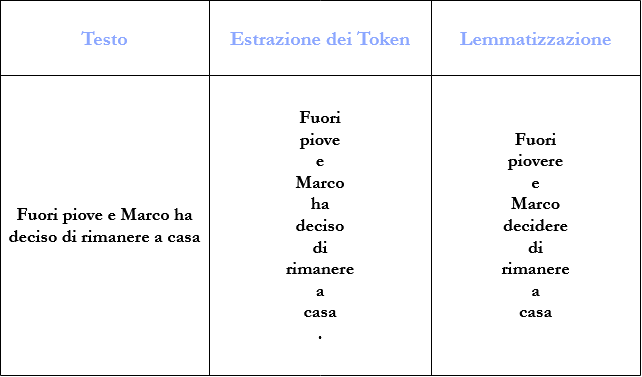
\includegraphics[width=0.8\textwidth]{img/analisi_lessicale.png}
        \caption{Analisi Lessicale}
        \label{fig:analisi_lessicale}
    \end{figure}
    
    \item \textbf{Analisi sintattica}: applica alle sequenze di token, ottenute tramite l’analisi lessicale, i principi della grammatica che genera il linguaggio nel quale è stato scritto il testo. Generalmente produce una struttura ad albero dove ad ogni nodo corrisponde o una parola o un costituente linguistico (frammento di frase), al quale corrisponderà una collocazione in una struttura gerarchica che nella sua radice copre l’intera frase. Si può dire che l’albero è la descrizione di tutte le relazioni grammaticali vigenti nella sequenza dei token in ingresso.
    L'insieme delle regole della sintassi prende nome di \textbf{regole di produzione} ed e strettamente collegato alla lingua.
    
    \begin{figure}[hbt!]
        \centering
        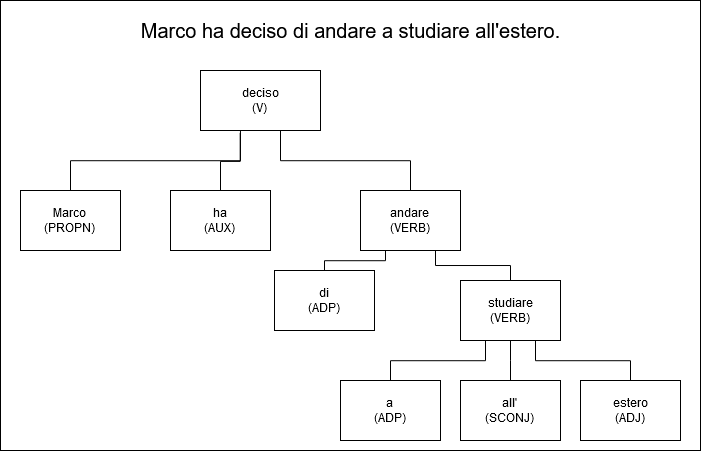
\includegraphics[width=0.8\textwidth]{img/analisi_sintattica.png}
        \caption{Analisi Sintattica}
        \label{fig:analisi_sintattica}
    \end{figure}
    
    \item \textbf{Analisi semantica}: si occupa di dare una spiegazione che descriva la relazione tra la frase e il mondo di riferimento (il "world model" nella figura \ref{fig:processo_nlp}).  L'analisi semantica è, pertanto, la ricerca del significato di un termine o di una frase. Non è sempre facile trovare il senso giusto delle parole. Spesso i termini hanno più significati (\textit{polisemici}) e occorre trovare quello giusto. Questo processo di selezione delle accezioni è detto \textbf{disambiguazione}. Le relazioni tra i concetti e i \textit{synset} consentono di costruire una struttura a rete detta \textbf{ontologia}. 
    In particolare si lavora su due livelli semantici differenti:
    
    \textbf{Semantica Lessicale}: studia il significato delle singole parole o di più termini, ovvero catene di parole il cui significato è diverso dalla somma dei significati delle singole parole (e.s. \textit{uscita d’emergenza}).
    
    \textbf{Semantica Frasale}: studia il significato di una frase, ponendo l’attenzione sulle interazioni tra i significati a livello delle parole. Prendiamo queste due frasi: \textit{Maria ha paura} vs. \textit{Maria sta giocando}. Maria ha lo stesso ruolo sintattico nei due casi (quello di soggetto) ma ha un diverso ‘ruolo semantico’: ha un ruolo attivo nell’attività di giocare, ma non nel caso di avere paura, che identifica uno stato emotivo che Maria vive involontariamente.
    
    A seconda del tipo di informazioni che si vogliono ottenere dai dati, è possibile usare una delle due tecniche di analisi semantica: \textit{text classification} o \textit{text extraction}. In particolare, in questa tesi sono stati trattati due task appartenenti alle queste due tecniche: \textbf{Topic Classification} per la Text Classification ed \textbf{Named Entity Recognition} per la Entity Extraction.
    
    \begin{figure}[hbt!]
        \centering
        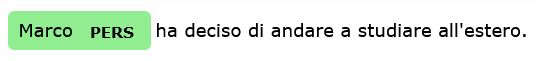
\includegraphics[width=0.8\textwidth]{img/analisi_semantica.png}
        \caption{Analisi Semantica: esempio di Named Entity Recognition}
        \label{fig:analisi_semantica}
    \end{figure}
    
    \item \textbf{Analisi pragmatica}: La dimensione pragmatica dell’analisi linguistica, secondo il filosofo americano Charles W. Morris, riguarda quegli aspetti che concernono l’azione indotta dall’uso del linguaggio. Studia il parlare in quanto forma di agire linguistico all’interno di una data situazione comunicativa. Molti enunciati, ad esempio, non veicolano informazioni, ma equivalgono ad azioni: “Scusami”, “Prometto”, “Si, lo voglio”, ecc.
    
    Nella forma logica, il significato delle parole viene messo in corrispondenza con il livello pragmatico (ovvero “cosa si aspetta da me la persona?”, “qual è  il suo scopo?”) e quindi, da un punto di vista applicativo, il sistema reagisce.  Le parole della forma logica rappresentano degli scopi e, dal punto di vista del modello, interpretare la forma logica e trasformarla in un’azione significa interpretare l’ultimo livello dell’analisi che è quello degli scopi che per l’utente ha quel testo.
\end{itemize}

\begin{figure}[hbt!]
    \centering
    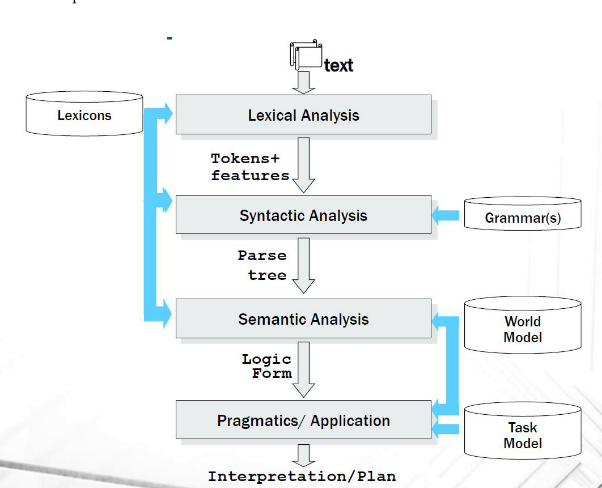
\includegraphics[width=1\textwidth]{img/processo_nlp.png}
    \caption{Il processo NLP}
    \label{fig:processo_nlp}
\end{figure}
\input{Capitoli_Interni/Capitolo2/Sottosezioni_1/3_Ambiguità}
\section{Campi d'applicazione}
Nella fase di sperimentazione riportata in questa tesi, come già citato, sono state proposte strategie risolutive ai problemi di \textit{Classificazione del testo} e \textit{Riconoscimento delle entità nominate}. L'attenzione è stata focalizzata su questi problemi poiché su di essi si fondano numerevoli sistemi software che, ormai, vengono utilizzati da quasi la totalità delle persone nella vita quotidiana e spesso sono impiegati anche a livello aziendale da diverse imprese. Alcuni esempi sono:\\\\
\textbf{Chatbots}\\
I chatbots sono una forma d'intelligenza artificiale programmata per interagire con gli esseri umani tanto da simulare loro stessi gli esseri umani. Capiscono la complessità del linguaggio naturale e trovano il significato reale della frase e imparano anche dalle loro conversazioni con gli umani migliorandosi con il tempo.\\\\
\\
\textbf{Completamento automatico nei motori di ricerca}\\
I motori di ricerca usano i loro enormi set di dati per analizzare ciò che i loro clienti stanno probabilmente digitando quando inseriscono determinate parole e suggeriscono le possibilità più comuni.\\\\
\textbf{Assistenti vocali}\\
Usano una complessa combinazione di riconoscimento vocale, comprensione del linguaggio naturale ed elaborazione del linguaggio naturale per capire ciò che gli esseri umani dicono e poi agire di conseguenza.\\\\
\textbf{Traduttore di lingua}\\
Questi strumenti di traduzione utilizzano anche la modellazione sequence to sequence che è una tecnica di elaborazione del linguaggio naturale. In precedenza, i traduttori di lingue usavano la traduzione automatica statistica (SMT) che significava analizzare milioni di documenti già tradotti da una lingua all'altra (dall'inglese all'hindi in questo caso) e poi cercare i modelli comuni e il vocabolario di base della lingua. Tuttavia, questo metodo non era così accurato rispetto alla modellazione Sequence to sequence.\\\\
\textbf{Analisi del sentimento}\\
Le aziende possono usare la sentiment analysis per capire come un particolare tipo di utente reagisce a un particolare argomento, prodotto, ecc. Possono usare l'elaborazione del linguaggio naturale, la linguistica computazionale, l'analisi del testo, ecc. per capire il sentimento generale degli utenti per i loro prodotti e servizi e scoprire se il sentimento è buono, cattivo o neutrale.\\\\
\\
\textbf{Controlli di grammatica}\\
Non solo possono correggere la grammatica e controllare l'ortografia, ma anche suggerire sinonimi migliori e migliorare la leggibilità complessiva del contenuto.\\\\
\textbf{Classificazione e filtraggio delle e-mail}\\
I servizi di posta elettronica utilizzano l'elaborazione del linguaggio naturale per identificare il contenuto di ogni e-mail con la classificazione del testo in modo che possa essere messo nella sezione corretta. In casi più avanzati, alcune aziende utilizzano anche software antivirus speciali con elaborazione del linguaggio naturale per scansionare le e-mail e vedere se ci sono modelli e frasi che possono indicare un tentativo di phishing sui dipendenti.

\section{Reti neurali per problemi linguistici}
\textit{In questa sezione viene trattata la storia dello sviluppo delle tecniche per il Natural Language Processing, per poi approfondire i concetti di percettrone, rete neurale e Deep Learning.}
\subsection{Primi approcci}
La storia della NLP viene fatta spesso partire dagli anni '50 del XX secolo, quando, nel famoso articolo \textit{Computing Machinery and Intelligence}\textsuperscript{\cite{10.1093/mind/LIX.236.433}}, Alan Turing propose il suo famoso test per valutare l'abilità di un computer di impersonare un umano durante una conversazione scritta in tempo reale. In realtà, quasi un decennio prima dell'uscita del suddetto articolo, si parlava già del concetto di \textit{Machine Translation}, un sottocampo della linguistica computazionale che studia l'uso di software per tradurre testi o discorsi da una lingua all'altra. Ma ciò è stato solo l'inizio della lunga storia dell'elaborazione del linguaggio naturale. Difatti, con il passare degli anni, si sono succeduti diversi approcci alla NLP. 

Nel 1957, il linguista americano Noam Chomsky, pubblicò \textit{Syntactic Structures}\textsuperscript{\cite{chomsky2002syntactic}}, opera che offrì un contributo fondamentale al problema introducendo la \textit{grammatica generativa}, insieme di regole che specificano in modo formale e ricorsivo le strutture sintattiche di un linguaggio. Ad esso, fino agli anni '80, anche a causa di un congelamento dei fondi USA destinati alla ricerca, seguirono sistemi NLP costituiti da strutture estremamente complesse di regole procedurali ed euristiche, che però a causa della loro rigidità risultarono incapaci di gestire l'estrema variabilità ed ambiguità del linguaggio naturale.

A cavallo tra gli anni '80 e '90, c'è stata una vera e propria rivoluzione dettata dall'introduzione degli algoritmi di machine learning per l'elaborazione del linguaggio. Si passò da sistemi \textit{rule-based} codificati manualmente a sistemi \textit{corpus-based} nei quali l'intervento umano diretto veniva limitato grazie all'apprendimento automatico a partire da uno o più corpus di riferimento. La maggior parte di questi approcci, utilizzati anche attualmente, forniscono un modo più avanzato per interpretare l'ambiguità e fornire ulteriori prove per la valutazione di una decisione. Algoritmi come gli alberi decisionali usano regole \textit{if-then} per ottenere il risultato ottimale e algoritmi probabilistici che sostengono la decisione presa dalla macchina fornendo una buona accuratezza.

Nel 2011, per la prima volta un algoritmo basato sul deep learning è stato applicato a differenti problemi di NLP, tra cui l’identificazione di entità e l’assegnazione di categorie morfologiche a parole, mostrando prestazioni sensibilmente migliori rispetto ad altri approcci rappresentativi dello stato dell’arte. Da allora, sono stati realizzati algoritmi sempre più complessi basati sul deep learning per affrontare problemi di NLP ancora non risolti o trattati in passato ma con risultati non soddisfacenti. 

Il Deep Learning è un ramo del Machine Learning, nel quale viene utilizzata una rete neurale con tre o più strati. Queste reti neurali tentano di simulare il comportamento del cervello umano permettendogli di "imparare" da grandi quantità di dati. Mentre una rete neurale con un solo strato può ancora fare previsioni approssimative, ulteriori strati nascosti possono aiutare a ottimizzare e raffinare la precisione.
\subsection{Percettrone}
Per comprendere il deep learning occorre prima chiarire il concetto relativo alle reti neurali artificiali (ANN). Il prototipo delle ANN sono le corrispettive biologiche: le reti neurali del cervello umano sono la sede della nostra capacità di comprendere l’ambiente e i suoi mutamenti e di fornire quindi risposte adattive calibrate sulle esigenze che si presentano. Un singolo neurone può ricevere simultaneamente segnali da diverse sinapsi e misurando il potenziale elettrico di tali segnali, stabilisce se è stata raggiunta la soglia di attivazione per generare a sua volta un impulso nervoso. Tale proprietà è implementata anche nelle reti artificiali.

Nel 1958 viene proposta da Rosenblatt la prima rete neurale \textbf{Perceptron}, fatta di un singolo strato con la seguente forma:

\begin{figure}[hbt!]
    \centering
    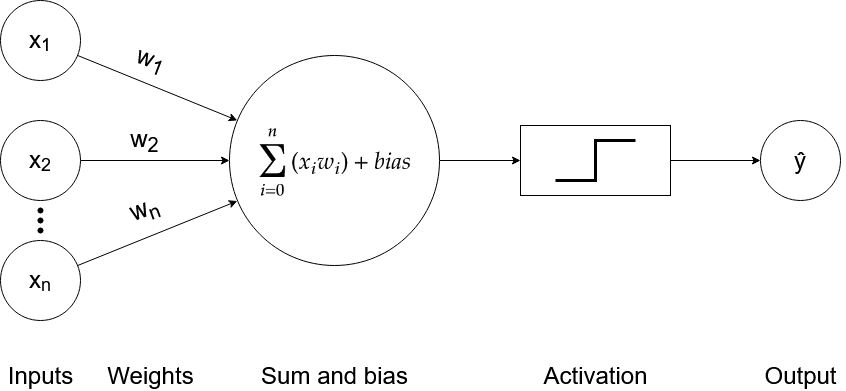
\includegraphics[width=0.9\textwidth]{img/perceptron.png}
    \caption{Percettrone}
    \label{fig:perceptron}
\end{figure}
L'idea di base è di usare diversi pesi per rappresentare l'importanza di ogni input. Se la somma di questi valori è maggiore di un certo valore di soglia, verrà presa una decisione come vero o falso (0 o 1). Nel dettaglio, un percettrone accetta gli input (\(x_1,x_2,...,x_n\)), li modera con dei valori di peso (\(w_1,w_2,...,w_n\)) ed applica loro una funzione di attivazione per produrre il risultato finale. 
La funzione di attivazione, solitamente, è definita come segue:
\begin{equation}
f(x) \ =\ \begin{cases}
        1 & if\ w\cdot x+b > 0\\
        0 & otherwise
    \end{cases}
\end{equation}
Dove:
\begin{itemize}
    \item \textbf{x}: è il vettore degli input
    \item \textbf{w}: è il vettore dei pesi
    \item \textbf{b}: è il bias, una costante che non dipende dai valori in input. Può essere pensato come un livello base di attivazione per l'output.
\end{itemize}

Una volta che abbiamo a disposizione un percettrone, si può cercare di istruirlo in modo che, dato un input \(x\), l'output \(f(x)\) sia quanto più vicino possibile a un dato valore \(g(x)\) scelto a priori.
Guardando la funzione di attivazione, notiamo che, essendo il vettore degli input non prevedibile ed il bias una costante, l'unico valore che è possibile modulare per far si che il percettrone restituisca il risultato desiderato è il vettore dei pesi \(w=(w_1,w_2,...,w_n)\). Infatti, nel cosiddetto \textit{apprendimento supervisionato}, man mano che la macchina elabora output, si procede a correggerla per migliorarne le risposte variando i pesi.

Le capacità computazionali di un singolo percettrone, però, sono limitate e le prestazioni che è possibile ottenere dipendono fortemente sia dalla scelta degli input, che dalla scelta della funzione che si desidera implementare.

\subsection{Deep Learning}
I modelli di Deep Learning vengono progettati per analizzare continuamente i dati con una struttura logica simile a quella utilizzata dagli esseri umani per trarre conclusioni. Per raggiungere questo obiettivo, le applicazioni di deep learning si avvalgono di una rete neurale artificiale a più strati, solitamente composte da: un livello di input, uno o più livelli nascosti (\textit{Hidden Layers}) e un livello di output. Ciascun nodo, o neurone artificiale, si connette ad un altro e ha un peso e una soglia associati. Se l'output di qualsiasi singolo nodo è al di sopra del valore di soglia specificato, tale nodo viene attivato, inviando i dati al successivo livello della rete. In caso contrario, non viene passato alcun dato al livello successivo della rete.

I percettroni multistrato vengono addestrati su coppie input-output e imparano a modellare le dipendenze tra ingresso e uscita. L'addestramento comporta la regolazione dei pesi o dei bias ad ogni strato della rete mediante l'utilizzo del backpropagation, un algoritmo di apprendimento supervisionato. La retropropagazione dell'errore cerca il valore minimo della funzione di errore nello spazio dei pesi usando la tecnica del \textit{gradient descent}. I pesi che minimizzano la funzione di errore sono poi considerati una soluzione al problema di apprendimento. 

Una prima caratteristica fondamentale di tali reti è che sono in grado di apprendere, in maniera autonoma e contestuale, le modalità con le quali combinare al meglio le informazioni ricevute per la risoluzione di un compito specifico.

Una seconda caratteristica è che, in maniera similare al cervello umano, sono in grado di imparare dalle loro esperienze, ossia di migliorare le proprie prestazioni nella risoluzione di un problema complesso in funzione della quantità di esempi con cui sono addestrati.
\begin{figure}[hbt!]
    \centering
    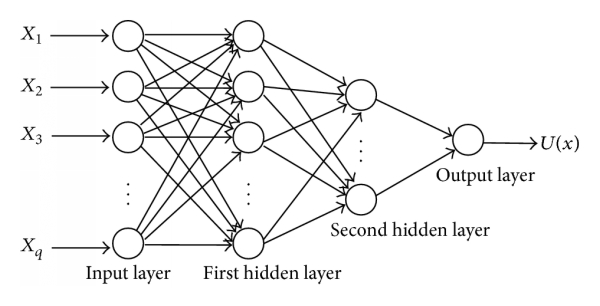
\includegraphics[width=0.8\textwidth]{img/ann.jpg}
    \caption{Esempio di una rete neurale artificiale}
    \label{fig:ann}
\end{figure}
\newpage
Tali reti sono in grado di elaborare, però, come input, solo dati numerici e non stringhe testuali. Questa è una delle motivazioni per le quali le prime applicazioni di successo del deep learning hanno riguardato il trattamento di immagini o segnali. Ad oggi sono state sviluppate diverse tecniche per la mappatura di contenuti testuali in vettori di numeri reali che permettono alle reti neurali di elaborare anche informazioni derivanti da corpus linguistici e pertanto essere impiegate per la risoluzione di task di Natural Language Processing.

Nei capitoli successivi tratteremo il concetto di \textbf{Word Embedding}, l'insieme delle tecniche il cui scopo è proprio quello di eseguire questa mappatura.



\section{Language Modeling}
Quando si lavora con un enorme corpus di dati testuali, è utile conoscere la probabilità con cui una sequenza di parole si succederà e quali particolari caratteristiche sono necessarie per capire questa dipendenza.

Il Language Modeling è il compito di capire questa distribuzione di probabilità su una sequenza di parole. Ciò aiuta a creare caratteristiche che possono distinguere tra frasi e frasi, secondo il contesto in cui appaiono.
I modelli linguistici interpretano questi dati alimentandoli attraverso un algoritmo che stabilisce regole per il contesto nel linguaggio naturale. A questo punto, il modello applica queste regole in compiti linguistici per prevedere o produrre nuove frasi. Il modello essenzialmente impara le caratteristiche del linguaggio di base e usa queste caratteristiche per capire nuove proposizioni.

Esistono diversi approcci probabilistici al language modeling, che variano a seconda dello scopo del modello linguistico. In questa tesi, è stato implementato un approccio al language modeling atto a modellare il testo in modo tale che questo possa essere convertito in un input numerico per una rete neurale artificiale. Nelle sezioni successive verrà approfondito proprio questo concetto, chiamato \textit{Word Embedding}, per poi discutere in particolar modo dei modelli \textit{GloVe}\textsuperscript{\cite{pennington-etal-2014-glove}}, \textit{BERT}\textsuperscript{\cite{devlin2019bert}} e \textit{USE}\textsuperscript{\cite{cer2018universal}}, utilizzati durante la fase di sperimentazione descritta nei capitoli successivi.
\subsection{Word Embedding}
Word embedding è il nome collettivo per definire un insieme di tecniche di language modeling e di apprendimento delle caratteristiche nell'elaborazione del linguaggio naturale in cui le parole o le frasi del vocabolario sono mappate in vettori di numeri reali. La necessità di questa pratica è nata con lo sviluppo delle reti neurali artificiali dato che, come accennato nella sezione riguardante il Deep Learning, esse possono elaborare soltanto input di natura numerica.

L'embedding si basa sul fatto che, in genere, le parole con un significato simile avranno rappresentazioni vettoriali che sono vicine tra loro nello spazio di incorporazione (anche se questo non è sempre stato il caso). Quando si codificano le parole, tipicamente l'obiettivo è quello di catturare qualche tipo di relazione in quello spazio, che sia il significato, la morfologia, il contesto o qualche altro tipo di connessione.

Molti word embedding sono creati sulla base della nozione introdotta dall'\textit{ipotesi distributiva} di Zellig Harris\textsuperscript{\cite{distributional_structure}}, che si riduce a una semplice idea che le parole che sono usate vicine l'una all'altra hanno tipicamente lo stesso significato.

Ciò diventa particolarmente utile quando i set di dati diventano sempre più grandi, perché con l’aumentare delle dimensioni spesso aumenta anche il numero di parole uniche. La presenza di molte parole usate raramente può causare problemi per un modello lineare; questo perché la quantità di possibili sequenze di parole aumenta, e i modelli che informano i risultati diventano più deboli. Ponderando le parole in modo non lineare e distribuito, questo modello può "imparare" ad approssimare le parole e quindi non essere fuorviato da eventuali valori sconosciuti. La sua "comprensione" di una data parola non è così strettamente legata alle parole immediatamente circostanti.

\subsection{Embedding statico: GloVe}
\textbf{GlobalVectors} (GloVe) è un modello assai noto che apprende i vettori o le parole dalle informazioni di co-occorrenza, ovvero la frequenza con cui compaiono insieme in grandi corpora di testo. GloVe è basato sul conteggio. In linea generale i modelli basati sul conteggio apprendono i vettori, operando una riduzione della dimensionalità sulla matrice di conteggio delle co-occorrenze.

Per prima cosa, si costruisce una grande \textbf{matrice di co-occorrenza} (parole x colonne), che contiene le informazioni sulla frequenza con cui ogni parola viene usata in un contesto. Il numero di contesti deve essere grande, poiché è essenzialmente di dimensioni combinatorie.

In seguito, tale matrice viene riscritta in forma algebrica e fattorizzata per ottenerne una dimensionalmente più piccola. Il risultato di questa operazione è una rappresentazione vettoriale per ogni parola.

L’addestramento può poi essere eseguito in due modi diversi: utilizzando il contesto per predire una parola target (utilizzando metodi noti come il BoW\textsuperscript{\cite{bow_article}} o il CBoW\textsuperscript{\cite{mikolov2013efficient}}) oppure usando una parola per predirre il contesto target (Skip-Gram\textsuperscript{\cite{skipgram}}).
% Precisamente, l'algoritmo GloVe consiste nei seguenti passi:
% \begin{enumerate}
%     \item Raccogliamo le statistiche di co-occorrenza delle parole in una forma di matrice di co-occorrenza di parole \(X\). Ogni elemento \(X_i_j\) di tale matrice rappresenta quanto spesso la parola \(i\) appare nel contesto della parola \(j\). Di solito scansioniamo il nostro corpus nel seguente modo: per ogni termine cerchiamo termini contestuali entro una certa area definita da una costante chiamata \(dimensione_finestra\) prima del termine e una \(dimensione_finestra\) dopo il termine. 
%     \clearpage
%     \begin{figure}[hbt!]
%         \centering
%         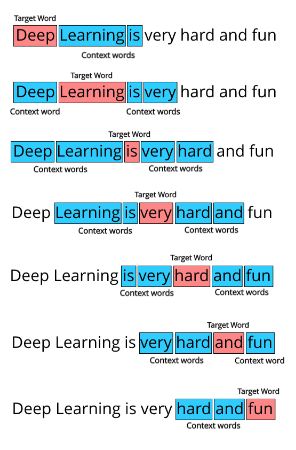
\includegraphics[width=0.5\textwidth]{img/context_window.png}
%         \caption{Context Window}
%         \label{fig:context_window}
%     \end{figure} \\
%     Inoltre diamo meno peso alle parole più lontane, di solito usando questa formula:
%     \begin{center}
%         \(decay=1/offset\)
%     \end{center}
    
%     \item Definiamo i vincoli per ogni coppia di parole:
%     \begin{center}
%         \(w^T_i w_j + b_i + b_j = log(X_i_j)\)
%     \end{center}
%     dove \(w_i\) è il vettore per la parola principale, \(w_j\) è il vettore per la \textit{context word}, \(b_j, b_j\) sono bias scalari rispettivamente per la parola principale e di contesto
    
%     \item Definiamo una funzione di costo:
%     \begin{center}
%         \[J = \sum_{i=1}^{V} \sum_{j=1}^{V} f(X_i_j)(w^T_i w_j + b_i + b_j - log(X_i_j))^2\]
%     \end{center}
%     Qui \(f\) è una funzione di ponderazione che ci aiuta a prevenire l'apprendimento solo da coppie di parole estremamente comuni. Gli autori di GloVe hanno scelto la seguente funzione:
%     \begin{center}
%         \[ f(X_i_j) = 
%           \begin{cases} 
%                 (\frac{X_i_j}{X_m_a_x})^\alpha & if X_i_j < X_m_a_x \\
%                 1 & otherwise
%             \end{cases}
%         \]
%     \end{center}
% \end{enumerate}
\subsection{Embedding contestualizzati: BERT}
I modelli statici come GloVe presentano diverse limitazioni:
\begin{itemize}
    \item L'uso di modelli linguistici molto superficiali. Questo significa che c'è un limite alla quantità di informazioni che possono catturare.
    \item Un'altra limitazione chiave è che questi modelli non prendono in considerazione il contesto della parola: questi modelli producono un solo embedding per ogni parola, combinando tutti i diversi sensi della parola in un unico vettore.
\end{itemize}
Alla fine del 2018 i ricercatori di Google AI Language hanno reso open-source una nuova tecnica per l'elaborazione del linguaggio naturale (NLP) chiamata \textbf{BERT (Bidirectional Encoder Representations from Transformers)} - una grande svolta che ha preso d'assalto la comunità del Deep Learning per le sue incredibili prestazioni. Il team di ricerca che ha lavorato dietro BERT lo descrive così:
\begin{center}
    \textit{"BERT sta per Bidirectional Encoder Representations from Transformers.  È progettato per pre-addestrare rappresentazioni bidirezionali profonde da testi non etichettati, condizionando congiuntamente il contesto sinistro e destro. Come risultato, il modello BERT pre-addestrato può essere messo a punto con un solo strato di output aggiuntivo per creare modelli all'avanguardia per una vasta gamma di compiti NLP."}
\end{center}
In primo luogo, BERT è basato sull'architettura \textbf{Transformer}, un modello proposto nel paper \textit{Attention is All You Need}\textsuperscript{\cite{vaswani2017attention}} che usa l'\textit{attenzione} (successore del modello sequence-to-sequence) per accelerare il processo di addestramento. In secondo luogo, BERT è pre-addestrato su un grande corpus di testo non etichettato che include l'intera \textbf{Wikipedia} (2.500 milioni di parole) e il Book Corpus (800 milioni di parole). In terzo luogo, BERT è un modello \textit{"profondamente bidirezionale"}. Bidirezionale significa che BERT apprende informazioni sia dal lato sinistro che da quello destro del contesto di un token durante la fase di formazione.

Il paper pubblicato dai creatori di Bert, presenta due modelli che si differenziano per le loro dimensioni: \begin{itemize}
    \item \textbf{BERT Base}: 12 strati (blocchi di trasformatori), 12 teste di attenzione e 110 milioni di parametri
    \item \textbf{BERT Large}: 24 strati (blocchi di trasformatori), 16 teste di attenzione e 340 milioni di parametri
\end{itemize}
\begin{figure}[hbt!]
    \centering
    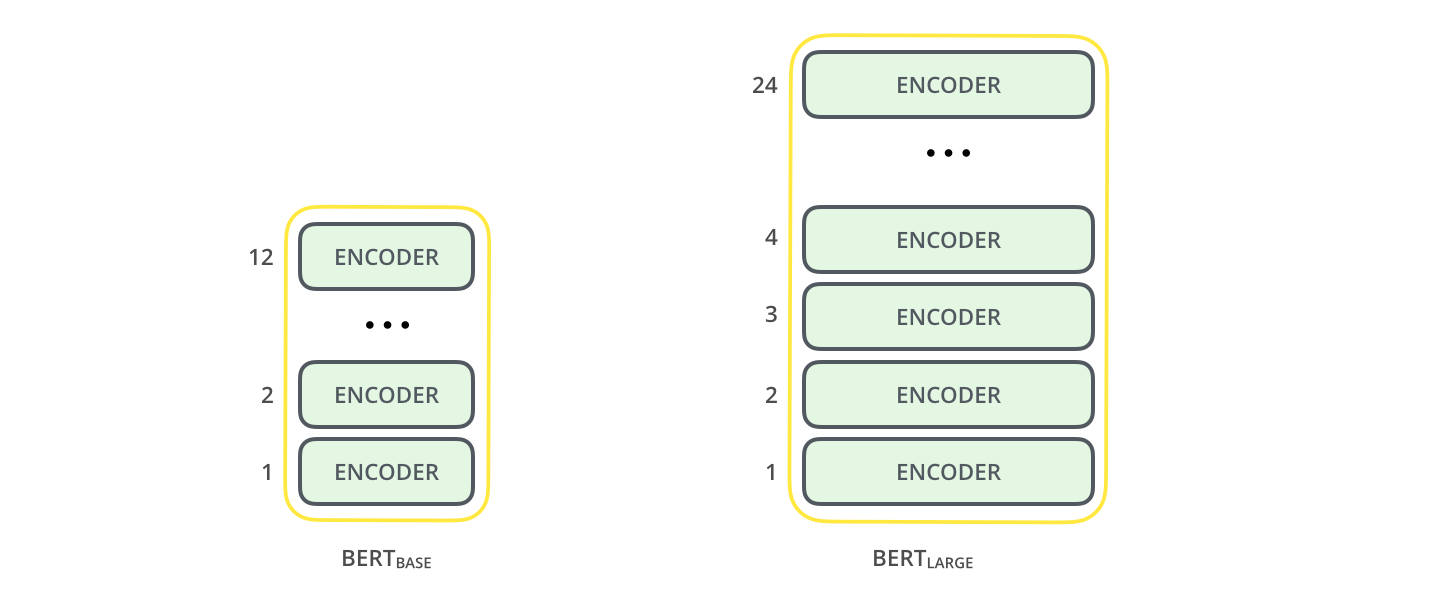
\includegraphics[width=1\textwidth]{img/bert_architecture.png}
    \caption{BERT Base e BERT Large}
    \label{fig:bert_architettura}
\end{figure}
\newpage
BERT è pre-addestrato su due compiti NLP:
\begin{itemize}
    \item \textbf{Masked Language Model}: Viene utilizzato per addestrare la capacità di BERT di catturare informazioni in maniera bidirezionale. Data una frase, il 15\% di essa viene \textit{mascherato} usando token speciali (ad esempio "[MASK]") e viene chiesto di prevedere la parola corretta che dovrebbe trovarsi in quella posizione. Durante l'addestramento di BERT viene utilizzata la seguente tecnica:
    \begin{enumerate}
        \item L'80\% delle volte le parole sono state sostituite con il token mascherato [MASK].
        \item Il 10\% delle volte le parole sono state sostituite con parole casuali.
        \item Il 10\% delle volte le parole sono rimaste invariate.
    \end{enumerate}
    \item \textbf{Next Sentence Prediction}: Questo è un task di classificazione binaria che viene utilizzato per addestrare BERT, in modo tale che quest'ultimo possa essere utilizzato in compiti nei quali è necessario sapere comprendere le relazioni che intercorrono tra le frasi. Il quesito posto è: date due frasi A e B prese da un corpus linguistico, determinare se la frase B segue la frase A nel testo oppure no.   
    \begin{enumerate}
        \item Per il 50\% delle coppie, la seconda frase sarebbe in realtà la frase successiva alla prima.
        \item Per il restante 50\% delle coppie, la seconda frase sarebbe una frase casuale dal corpus.
    \end{enumerate}
\end{itemize}
\subsection{Embedding contestualizzati: Universal Sentence Encoder}
BERT è uno strumento molto potente ma, proprio per questo motivo non è la soluzione migliore quando si tratta di utilizzarlo su dispositivi con memoria o potenza di calcolo limitata. È da questa idea che nasce il progetto proposto da \citet{cer2018universal}.

L'\textbf{Universal Sentence Encoder (USE)} codifica il testo in vettori ad alta dimensione che possono essere utilizzati per la classificazione del testo, la similarità semantica, il clustering e altri compiti del Natural Language Processing. L'idea è quella di progettare un codificatore che riassuma qualsiasi frase data in un'embedding a 512 dimensioni. Si usa questo stesso embedding per risolvere compiti multipli e in base agli errori che vengono fatti su di essi, aggiorniamo la codifica della frase. Poiché essa deve lavorare su più compiti generici, catturerà solo le caratteristiche più informative e scarterà il rumore. L'intuizione è che, così facendo, il risultato possa essere universalmente compatibile per essere incorporato a diversi task anche molto distanti tra loro.

L'Universal Sentence Encoder pre-addestrato è disponibile pubblicamente in \textbf{Tensorflow-hub}. Viene fornito in due varianti:
\begin{enumerate}
    \item \textbf{Transformer Encoder}: In questa variante, usiamo la parte encoder dell'architettura originale del transformer. L'architettura consiste di 6 strati di trasformatori impilati. Ogni strato ha un modulo di self-attention seguito da una rete feed-forward.
    \item \textbf{Deep Averaging Network}: Word embeddings e i bi-grammi presenti in una frase sono mediate insieme. Poi attraversano una DNN profonda a 4 strati feed-forward per ottenere in uscita un'embedding per l'intera frase a 512 dimensioni. Le embeddings per le parole e i bi-grammi sono apprese durante l'addestramento.
\end{enumerate}
I due modelli hanno un compromesso di accuratezza e richiesta di risorse computazionali. Mentre quello con un codificatore Transformer ha una maggiore precisione ma è computazionalmente più intenso, quello con codifica DAN usa meno memoria con un leggero compromesso a livello di precisione.

Il modello di codifica è progettato per essere il più generale possibile. Ciò viene realizzato utilizzando l'apprendimento multi-task in cui un singolo modello di codifica viene addestrato per risolvere più compiti diversi. I tasks supportati includono: un compito simile a Skip-Thought (\citet{NIPS2015_f442d33f}) per l'apprendimento non supervisionato da un testo corrente arbitrario; un task di input-risposta conversazionale (\citet{henderson2017efficient}); e compiti di classificazione per l'addestramento su dati supervisionati. Il compito Skip-Thought sostituisce il LSTM (\citet{Hochreiter1997LongSM}) usato nella formulazione originale con un modello un modello basato sull'architettura Transformer. 

\chapter{Una soluzione distribuita} \label{sol_distribuita}
%cappello introduttivo
In questo capitolo verranno presentate le tecnologie coinvolte nello sviluppo della soluzione utilizzata durante la fase di sperimentazione, focalizzandosi particolarmente sui concetti di calcolo distribuito e Transfer Learning.
%sezioni
\section{Calcolo Distribuito}
Questa tesi nasce dall'idea di sperimentare ed analizzare le prestazioni offerte dal framework Spark NLP eseguendolo in ambiente distribuito. Ma cosa è Spark NLP? Su cosa si basa? E perché usare un ambiente distribuito? Per rispondere a queste domande bisogna partire descrivendo cosa è il calcolo distribuito.

Wikipedia definisce il calcolo distribuito come \textit{<<un campo dell'informatica che studia i sistemi distribuiti, ovvero sistemi che consistono in numerosi computer che interagiscono tra loro attraverso una rete al fine di raggiungere un obiettivo comune>>}. In altre parole, i sistemi distribuiti sono una collezione di componenti indipendenti situati su diverse macchine che, messi in comunicazione tra loro, interagiscono al fine di raggiungere un obiettivo comune fornendo importanti vantaggi a chi li implementa, come: aumento delle prestazioni, tolleranza agli errori e diminuzione del carico. Un sistema distribuito può consistere in qualsiasi numero di possibili configurazioni, come mainframe, personal computer, workstation, minicomputer e così via. L'obiettivo è quello di far funzionare tale rete come un singolo computer. I motivi principali per cui utilizzare un sistema distribuito sono:
\begin{itemize}
    \item \textbf{Affidabilità}: il sistema generalmente non subisce interruzioni se una singola macchina si guasta.
    \item \textbf{Scalabilità}: è facile e generalmente poco costoso aggiungere altri nodi e funzionalità se necessario.
    \item \textbf{Performance}: sono estremamente efficienti perché i carichi di lavoro possono essere suddivisi e inviati a più macchine.
\end{itemize}
La progettazione di questi sistemi è comunque un lavoro dispendioso. Nonostante i considerevoli benefici che essi portano, questi ultimi potrebbero non ripagare i costi di realizzazione. Le maggiori sfide che un sistema distribuito potrebbe incontrare si dividono in:
\begin{itemize}
    \item \textbf{Scheduling}: decidere quali lavori devono essere eseguiti, quando devono essere eseguiti e dove devono essere eseguiti. 
    \item \textbf{Latenza}: spesso potrebbero essere incontrati dei problemi a livello di latenza, che creano inconvenienti a livello di efficienza e consistenza dei dati. Questo motivo porta i team a fare compromessi tra disponibilità, coerenza e latenza. 
    \item \textbf{Osservabilità}: raccogliere, elaborare, presentare e monitorare le metriche di utilizzo dell'hardware per grandi sistemi è una sfida significativa
\end{itemize}
Nello specifico, in questo progetto è stato utilizzato un tipo di sistema distribuito chiamato \textbf{Cluster}. Quando si parla di cluster si intende un sistema di computer connessi tramite una rete con lo scopo di distribuire una elaborazione (parallelizzabile) tra i computer che compongono il cluster.
\section{Hadoop}
I big data sono un'industria a sé ma sono anche al centro delle strategie di molte aziende che desiderano migliorare la gestione dei clienti, il marketing e lo sviluppo. É quando si considerano campi dove la quantità di informazioni che girano intorno ad essi è così estesa, che entrano in gioco i sistemi distribuiti e strumenti come Hadoop che sono essenziali per gestire un notevole afflusso di dati. Proprio per questo motivo, in questa tesi, alla base del sistema distribuito implementato all'interno del progetto, c'è proprio Apache Hadoop. 
\subsection{Cosa è Hadoop}
Hadoop\footnote{Apache Hadoop: \href{https://hadoop.apache.org/}{https://hadoop.apache.org/}} è stato creato dalla Apache Software Foundation\footnote{Apache Software Foundation \href{https://www.apache.org/}{https://www.apache.org/}} ed è stato prodotto nei primi anni 2000 per rispondere alla crescita dei motori di ricerca come Yahoo e Google. Nato da Doug Cutting e Michael Cafarella, il progetto prese il nome dall'elefante giocattolo di uno degli sviluppatori. Hadoop è stato rilasciato come progetto open-source nel 2008 e poi nel 2012 dalla Apache Software Foundation. Oggi, Hadoop è composto da librerie open-source destinate ad elaborare grandi insiemi di dati su migliaia di computer in cluster.

Si tratta di un framework per l'esecuzione di applicazioni su grandi cluster costruiti con hardware di largo consumo a basso costo. Hadoop fornisce in modo trasparente applicazioni sia per l'affidabilità che per il trasferimento dei dati e consiste di quattro moduli principali:
\begin{itemize}
    \item \textbf{Hadoop Common}: utilities che supportano gli altri moduli Hadoop.
    \item \textbf{Hadoop Yet Another Resource Negotiator (YARN)}: Un framework per lo scheduling dei job e la gestione delle risorse del cluster
    \item \textbf{Hadoop Distributed File System (HDFS)}: Un file system distribuito che fornisce un accesso ad alta velocità ai dati delle applicazioni.
    \item \textbf{Hadoop MapReduce}: Un sistema basato su YARN per l'elaborazione parallela di grandi insiemi di dati.
\end{itemize}

Nella fase di sperimentazione, Hadoop è stato utilizzato per implementare un file system distribuito attraverso il quale, le macchine appartenenti al cluster possono processare i dataset di addestramento e di test in maniera distribuita. Per chiarire questo concetto abbiamo però bisogno di introdurre il funzionamento di HDFS, MapReduce e YARN.
\subsection{Hadoop Distributed File System} \label{hdfs}
L'Hadoop Distributed File System (HDFS)\footnote{Documentazione HDFS: \href{https://hadoop.apache.org/docs/r1.2.1/hdfs\_user\_guide.html}{https://hadoop.apache.org/docs/r1.2.1/hdfs\_user\_guide.html}} è un file system gerarchicho e distribuito progettato per funzionare su hardware di base. Ha molte somiglianze con i file system distribuiti esistenti. Tuttavia, le differenze con essi sono significative. HDFS è altamente tollerante agli errori ed è progettato per essere implementato su hardware a basso costo. Inoltre, fornisce un accesso ad alta velocità ai dati delle applicazioni ed è adatto al i software che utilizzano grandi set di dati.

L'architettura di HDFS è di tipo master/slave composta da un singolo master (\textbf{NameNode}) e un numero arbitrario di slaves/workers (\textbf{DataNode}), solitamente uno per ogni nodo del cluster. HDFS espone un namespace del file system e permette ai dati dell'utente di essere memorizzati in file, i quali sono divisi in uno o più blocchi che verranno memorizzati in un insieme di DataNodes. 

Il NameNode è un master server che possiede l'albero di tutte le directory del filesystem e gestisce operazioni di apertura, rinominazione e chiusura dei file. Risponde alla richiesta del client restituendo una lista di server DataNode pertinenti dove risiedono i dati. Qualsiasi cambiamento al namespace del file system o alle sue proprietà viene registrato dal NameNode. 

I DataNode contengono multipli blocchi di dati e la loro responsabilità è quella di eseguire operazioni di creazione, eliminazione e replicazione dei blocchi sotto istruzioni del NameNode. Una volta che il NameNode fornisce la posizione dei dati, le applicazioni client possono parlare direttamente con un DataNode mentre, replicando i dati, le istanze DataNode possono parlare tra loro.

Per garantire una buona tolleranza ai guasti, i blocchi di un file vengono replicati. La dimensione del blocco e il fattore di replica sono configurabili per ogni file e un'applicazione può specificare il numero di repliche al momento della sua creazione o cambiarlo in seguito.
\begin{figure}[hbt!]
    \centering
    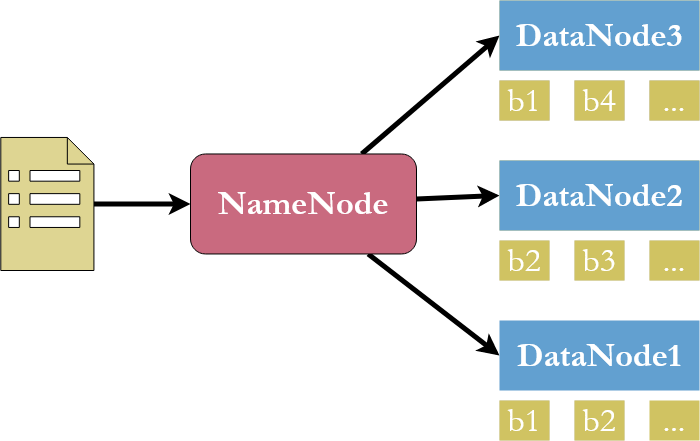
\includegraphics[width=0.7\textwidth]{img/hdfs.png}
    \caption{Architettura HDFS}
    \label{fig:hdfs_architettura}
\end{figure}

\subsection{MapReduce}
MapReduce\footnote{Documentazione MapReduce \href{https://hadoop.apache.org/docs/r1.2.1/mapred\_tutorial.html}{https://hadoop.apache.org/docs/r1.2.1/mapred\_tutorial.html}} è un framework per la creazione di applicazioni in grado di elaborare grandi quantità di dati in parallelo, permettendo una scalabilità massiccia su centinaia o migliaia di server in un cluster Hadoop. É stato reso popolare come modello di programmazione nel 2004 da Jeffery Dean e Sanjay Ghemawat di Google. Nel loro articolo \textit{MapReduce: simplified data processing on large clusters}\textsuperscript{\cite{pub62_mapreduce}} hanno discusso l'approccio di Google alla raccolta e all'analisi dei dati dei siti web per l'ottimizzazione della ricerca. Successivamente implementato da Apache, è diventato uno dei componenti principali del progetto Hadoop, nel quale, come il componenente HDFS è il responsabile della memorizzazione dei file, MapReduce si occupa di processare questi ultimi.

L'algoritmo implementato prende il nome dalle principali funzioni da cui è composto:
\begin{itemize}
    \item \textbf{Map}: trasforma i dati ricevuti in input in tuple formate da coppie chiave/valore.
    \item \textbf{Reduce}: prende in input l'output generato da Map e combina le coppie chiave-valore in un insieme più piccolo di tuple.
\end{itemize}
Tra le funzioni Map e Reduce avvengono operazioni di \textit{sorting} e \textit{shuffling} che si occupano di ordinare e raggruppare per chiave l'output di Map e fornirlo come input a Reduce.

MapReduce lavora secondo il principio del \textit{divide et impera}, suddividendo l'operazione di calcolo in diverse parti che verranno processate in modo autonomo per poi ricomporle (o ridurle) in un unico risultato finale. Queste parti sono dette \textit{jobs} e sono formate da sorgente di input, destinazione dei dati e le funzioni Map e Reduce.

Generalmente, l'algoritmo viene eseguito sugli stessi nodi su cui risiede HDFS, il che significa che ognuno di essi viene utilizzato sia per il calcolo che per lo storage. Il vantaggio di una tale configurazione è che i compiti possono essere programmati sui nodi dove risiedono i dati e quindi risulta un'elevata larghezza di banda aggregata in tutto il cluster.
\begin{figure}[hbt!]
    \centering
    \includegraphics[width=1\textwidth]{img/mapreduce.png}
    \caption{Algoritmo MapReduce}
    \label{fig:mapreduce}
\end{figure}\\

Come e da chi vengono gestite internamente queste operazioni? MapReduce, a livello architetturale, presenta due componenti: 
\begin{itemize}
    \item \textbf{Job Tracker}: si occupa della gestione delle risorse (CPU e memoria) e del ciclo di vita di un job MapReduce. Il JobTracker distribuisce il lavoro tra i nodi più vicini che contengono i dati da elaborare; nel caso in cui un nodo non possa ospitare il task, si fa poi carico della schedulazione del job nonché della ripetizione dell’esecuzione dei singoli task di MapReduce che si trovano in uno stato di errore. 
    \item \textbf{Task Tracker}: Sono le componenti che girano sui singoli nodi e che eseguono effettivamente i task sotto la direzione del JobTracker.
\end{itemize}

Cosa rende questo framework così importante? I benefici che porta sono notevoli e, alla sua nascita, portò grande innovazione nel campo del calcolo distribuito. I due principali vantaggi che questa tecnologia offre sono:
\begin{enumerate}
    \item \textbf{Elaborazione parallela}: l'intero lavoro è diviso in job che vengono elaborati in modo parallelo simultaneamente, riducendo drasticamente i tempi di esecuzione.
    \item \textbf{Località dei dati}: invece di spostare tutti i dati per l'elaborazione, il processo completo viene spostato su ogni nodo. Col crescere del quantitativo di dati da processare, può diventare difficile spostarli da un posto all'altro e quindi questa tecnica è considerata un'alternativa assai vantaggiosa.
\end{enumerate}


\subsection{YARN} \label{yarn}
Quando i dati hanno cominciato a diventare sempre più grandi, Hadoop File System è stato in grado di immagazzinarli, ma MapReduce è diventato un collo di bottiglia nelle prestazioni. Questo perché, in Hadoop 1.x, il JobTracker si occupava sia della gestione delle risorse, sia dell'elaborazione dei dati. Per questo motivo, in Hadoop 2.0\footnote{Hadoop 2.0 changelog: \href{https://hadoop.apache.org/release/2.2.0.html}{https://hadoop.apache.org/release/2.2.0.html}} è stato introdotto \textit{YARN\footnote{YARN docs: \href{https://hadoop.apache.org/docs/current/hadoop-yarn/hadoop-yarn-site/YARN.html}{https://hadoop.apache.org/docs/current/hadoop-yarn/hadoop-yarn-site/YARN.html}} (Yet Another Resources Navigator)} che separa il livello di gestione delle risorse dal livello di elaborazione. L'idea fondamentale di YARN è di dividere queste funzionalità in processi separati:
\begin{itemize}
    \item \textbf{ResourceManager}: è il processo master di YARN ed è responsabile dell'assegnazione e della gestione delle risorse tra tutte le applicazioni. Ogni volta che riceve una richiesta di elaborazione, la inoltra al gestore del nodo corrispondente (NodeManager) e alloca le risorse per il completamento della richiesta. Viene suddiviso in ulteriori due componenti:
    \begin{itemize}
        \item \textbf{Scheduler}: esegue la pianificazione in base all'applicazione assegnata e alle risorse disponibili. Non esegue altri compiti come il monitoraggio o il tracking e non garantisce un riavvio se un compito fallisce. 
        \item \textbf{ApplicationManager}: è responsabile di dell'accettazione dell'applicazione e della negoziazione del primo container\footnote{Per container si intende un insieme di risorse fisiche come RAM, core di CPU e disco su un singolo nodo.} dal gestore delle risorse. Riavvia anche il container ApplicationMaster se un job fallisce.
    \end{itemize}
    \item \textbf{NodeManager}: è l'agente del framework per ogni macchina ed è responsabile del monitoraggio del loro utilizzo delle risorse (cpu, memoria, disco, rete) e della segnalazione al ResourceManager. Si registra con il ResourceManager e invia \textit{heartbeat} (segnali) con lo stato di salute del nodo. Monitora l'uso delle risorse, esegue la gestione dei log e uccide anche un container in base alle indicazioni del gestore delle risorse. 
    \item \textbf{ApplicationMaster}: è una libreria specifica del framework e ha il compito di negoziare le risorse dal ResourceManager e lavorare con i NodeManager per eseguire e monitorare i job.
\end{itemize}

\begin{figure}[ht!]
    \centering
    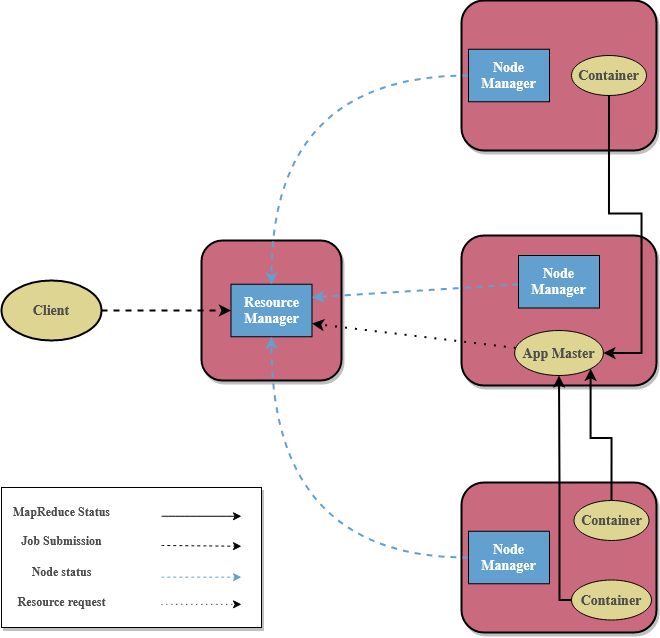
\includegraphics[width=0.8\textwidth]{img/yarn.png}
    \caption{Architettura YARN}
    \label{fig:yarn}
\end{figure}
\clearpage
%  \subsection{Utilizzo di Hadoop} \label{uso_hadoop}
Descritte le componenti HDFS e MapReduce, è possibile proseguire con illustrando come Hadoop è stato inserito all’interno del progetto di Tesi.

Come citato precedentemente, l’obiettivo ultimo è quello di testare soluzioni per la risoluzione di task di NLP in ambiente distribuito. Per fare ciò è stato configurato un database distribuito HDFS su di un cluster di 3 macchine connesse tre loro. Così facendo, tutte le macchine del sistema hanno accesso ai file contenenti i dataset di addestramento e di testing, ed ai modelli utilizzati (sia preaddestrati che allenati al momento della sperimentazione). Nel dettaglio, il nodo master del cluster ospita il NameNode, che si occupa della gestione del namespace del file system, mentre su ognuna delle altre macchine è stato invece allocato un processo DataNode, con lo scopo di delegare loro la manipolazione dei blocchi di dati secondo le indicazioni del NameNode.

Il concetto di MapReduce è invece ereditato da Apache Spark, framework su cui si basa Spark NLP, ovvero il soggetto di questo lavoro. Spark, come avviene con MapReduce, suddivide il processo in jobs e distribuisce questi ultimi tra i nodi del cluster migliorando le proprie prestazioni in fatto di distribuzione del carico e velocità di esecuzione. Nel capitolo successivo si entrerà nel dettaglio del funzionamento di Spark e di come è stato implementato all’interno del progetto.
\section{Apache Spark} \label{spark}
Apache Spark\footnote{Apache Spark:  \href{https://spark.apache.org}{https://spark.apache.org}} nasce come un progetto di ricerca al \href{https://amplab.cs.berkeley.edu/}{UC Berkeley AMPLab} nel 2009 per poi essere reso pubblico sotto forma di progetto open source nel 2010. Acquistato dall'Apache Software Foundation nel 2013, ad oggi è uno dei framework più utilizzati nel campo delle elaborazioni distribuite di grandi quantità di dati, con alle spalle una comunità di centinaia di sviluppatori e centinaia di organizzazioni.
\subsection{Cosa è Spark}
Apache Spark è un motore multilingue per la automazione di ingegneria dei dati, scienza dei dati e apprendimento automatico su macchine a nodo singolo o cluster. La peculiarità di Apache Spark è la sua capacità di elaborare set di dati di grandi dimensioni in maniera efficiente, distribuendo attività di elaborazione dati su più computer, anche integrando Hadoop YARN e HDFS. Questi attributi sono fondamentali per il mondo dei big data e del machine learning.

All'epoca della nascita di questo progetto, Hadoop MapReduce era il motore di programmazione parallela predominante per i cluster, essendo il primo sistema open source ad affrontare l'elaborazione dei dati su migliaia di nodi. L'AMPlab aveva lavorato con molti dei primi utenti di MapReduce per capire i benefici e gli svantaggi di questo nuovo modello di programmazione ed era quindi in grado di sintetizzare una lista di problemi attraverso diversi casi d'uso e iniziare a progettare piattaforme di calcolo più generali. Spark pertanto nasce prendendo i pregi di MapReduce ed introducendo nuove funzionalità che, ad oggi, lo hanno reso uno dei framework più solidi nell'ambito dei big data:
\begin{itemize}
    \item Spark supporta l’elaborazione in memoria centrale per migliorare le prestazioni delle applicazioni, a differenza di MapReduce che deve riportare i dati sul disco dopo ogni azione Map o Reduce.
    \item Il suo predecessore poteva essere implementato soltanto utilizzando il linguaggio Java. Spark, invece, fornisce connessioni native per i linguaggi di programmazione Java, Scala, Python e R e supporta operazioni SQL. 
    \item Può elaborare grafi ed è anche dotato di una propria libreria di machine learning. Grazie alle sue alte prestazioni, è possibile utilizzarlo sia per l'elaborazione in batch sia per l'elaborazione simil real-time. 
    \item Sfrutta il paradigma del Transfer Learning (il riutilizzo di un modello pre-addestrato su un nuovo problema). 
    \item Permette di elaborare dei dati da vari repository come Hadoop Distributed File System (HDFS), database NoSQL e Apache Hive utilizzando le API di storage di dell'ecosistema Hadoop.
    \item In MapReduce, ogni operazione è indipendente dall'altra e Hadoop non ha idea di quale verrà dopo. Spark, invece, utilizza un modello di programmazione completamente innovativo basato su grafi diretti aciclici (DAGs).
\end{itemize}

\subsection{Architettura}
L'architettura di Apache Spark si ispira fortemente a quella di Hadoop. Difatti, presenta una struttura gerarchica \textbf{Master-Slaves} dove il nodo master che gestisce i nodi in esecuzione e controlla l’amministratore del cluster. 

All'interno del nodo master viene istanziato un \textit{driver}, processo che si occupa di distribuire il codice dell’utente tra i nodi e convertirlo in più attività (\textit{jobs}). Il driver distribuisce questi compiti sui nodi slave (worker) e organizza la loro esecuzione.  Le applicazioni Spark vengono eseguite come serie indipendenti di processi in ambiente distribuito, coordinate dallo \textbf{SparkContext}, un processo che funziona come una porta d'accesso a tutte le funzionalità di Spark.

I \textbf{nodi worker} eseguono le attività assegnate dal driver su questi nodi. Eseguti i jobs assegnati, restituiscono il risultato allo SparkContext. 
È però necessario implementare un gestore del cluster o \textbf{cluster manager} (Spark Standalone Cluster Manager, Hadoop Yarn, Apache Mesos, Kubernetes) per mediare tra i workers e driver. 
\begin{figure}[hbt!]
    \centering
    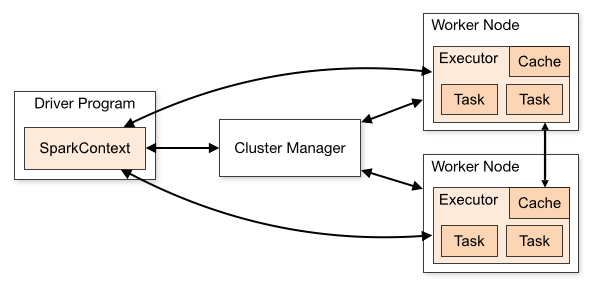
\includegraphics[width=1\textwidth]{img/sparkarchitecture.png}
    \caption{Architettura Spark}
    \label{fig:spark_architettura}
\end{figure}\\

% Spark può essere eseguito in due modalità:
% \begin{itemize}
%     \item \textbf{Cluster Mode}: il cliente che presenta l'applicazione Spark avvierà il driver e manterrà lo SparkContext. Quindi, fino a quando l'esecuzione del lavoro non sarà finita, la gestione dei jobs sarà svolta dal driver. Inoltre, il client deve rimanere sempre in contatto con il cluster: il client dovrà essere online fino a quando quel particolare processo non sarà completato.
%     \item \textbf{Client Mode}: il driver Spark o il master dell'applicazione Spark verrà avviato in una qualsiasi delle macchine worker. Quindi, il client che sta presentando l'applicazione può presentare l'applicazione e può o andare via dopo aver avviato l'applicazione o continuare con qualche altro lavoro. Questo meccanisco è anche chiamato \textit{Fire and Forget}.
% \end{itemize}
\subsection{Spark RDD e DataFrame} \label{rdd_df}
Il motore Spark usa principalmente set di \textit{Resilient Distributed Dataset (RDD)} come tipo di dati sottostante. Gli RDD sono raccolte di elementi a tolleranza di errore che possono essere distribuiti tra più nodi in cluster e lavorati in parallelo. Hanno una struttura progettata per nascondere la complessità computazionale agli utenti: non hanno bisogno di definire dove vengono inviati file specifici, quali risorse di calcolo verranno utilizzate per archiviare o recuperare i file. Sono altamente resilienti, cioè sono in grado di superare rapidamente qualsiasi problema poiché gli stessi pezzi di dati sono replicati su più nodi esecutori, così, anche se un nodo fallisce, un altro elaborerà comunque i dati.

Ci sono due modi per creare RDD - parallelizzando una collezione esistente nel programma driver, o facendo riferimento a un set di dati in un sistema di storage esterno, come un file system condiviso, HDFS, HBase, ecc. Con gli RDD, si possono eseguire due tipi di operazioni:
\begin{itemize}
    \item \textbf{Transformations}: prendono RDD come input e producono uno o più RDD come output. Ogni volta creano un nuovo RDD poiché essi sono immutabili. 
    \item \textbf{Actions}: operazioni Spark RDD che danno valori non RDD. I valori dell'azione sono memorizzati nel driver o nel sistema di archiviazione esterno. Un'azione è uno dei modi per inviare dati da Executer al driver.
\end{itemize}
\begin{figure}[hbt!]
    \centering
    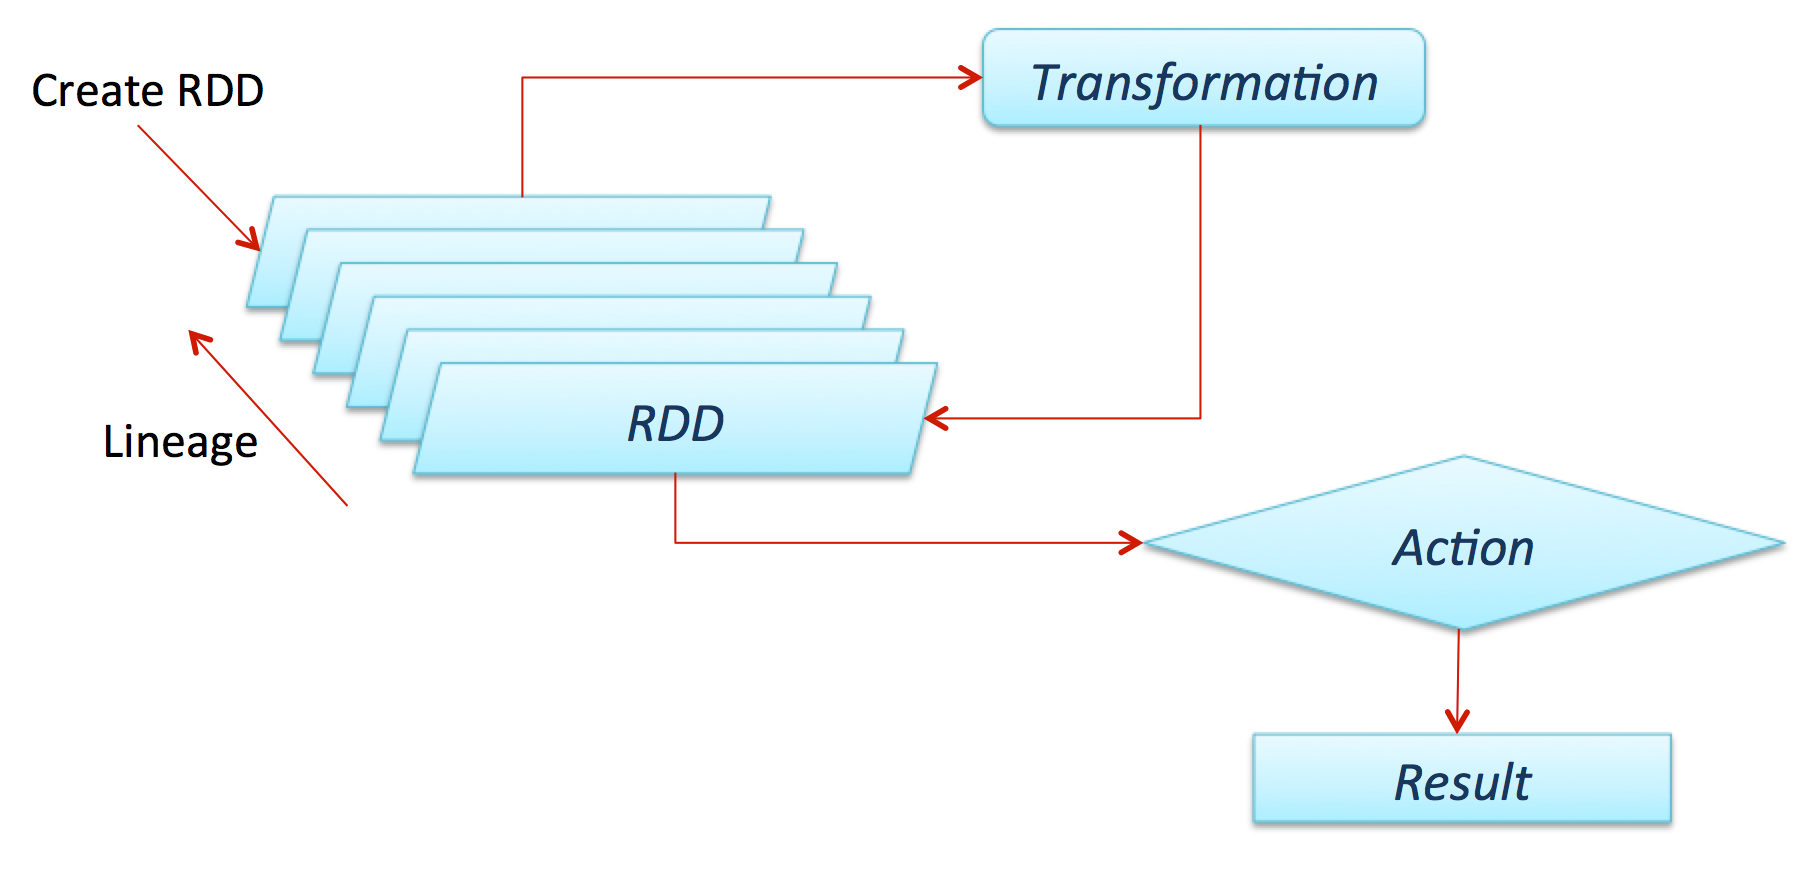
\includegraphics[width=1\textwidth]{img/spark_rdd.png}
    \caption{Operazioni su RDD}
    \label{fig:spark_rdd}
\end{figure}

Nel progetto di Tesi è stato però utilizzato un altro tipo astrazione presente in Spark per memorizzare dati, i \textit{DataFrame}. Sono implementati come degli RDD, pertanto sono anch'essi una collezione di dati distribuiti. La differenza sta nel fatto che sono organizzati in colonne nominate, come avviene nelle tabelle dei database relazionali. Un'altra caratteristica di DataFrame è che le operazioni sono ottimizzabili da Spark mentre le operazioni su RDD sono imperative e passano attraverso le trasformazioni e le azioni in ordine. Questo perfezionamento viene eseguito da un ottimizzatore di query, \textit{Catalyst Optimizer}, che supporta sia l'ottimizzazione basata sulle regole che quella basata sui costi. Nell'ottimizzazione basata su regole, usa un insieme di regole per determinare come eseguire la query. L'ottimizzazione basata sul costo trova il modo più adatto per eseguire l'istruzione. Nell'ottimizzazione basata sui costi, vengono generati più piani utilizzando le regole e poi viene calcolato il loro costo.
\begin{figure}[hbt!]
    \centering
    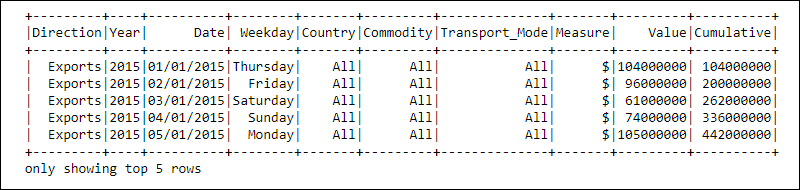
\includegraphics[width=1\textwidth]{img/dataframe_example.png}
    \caption{Esempio di struttura di un DataFrame}
    \label{fig:dataframe_example}
\end{figure}

Durante la fare di sperimentazione, sono stati utilizzati DataFrame per memorizzare i record presenti nei dataset ed effetturare operazioni su di essi. I DataFrame sono stati popolati utilizzando metodi implementati all'interno della struttura dati che permettono di estrarre informazioni da file di diversi formati. Nello specifico sono stati utilizzati per leggere dati da file in formato CSV e CoNLL '03.
\subsection{Directed Acyclic Graphs in Spark}
Con tutti i vari job, Spark crea un flusso logico di operazioni, che è noto come \textbf{Directed Acyclic Graph (DAG)}. In Spark, un DAG è un grafo diretto aciclico dove i \textit{vertici} rappresentano le strutture dati (RDD o DataFrame) e gli \textit{archi} rappresentano l'operazione da applicare su di esse. Alla chiamata di un'azione, il DAG creato viene sottoposto al \textit{DAGScheduler} che divide ulteriormente il grafo nelle fasi da svolgere per portare a termine il compito. Questo aiuta a: ridurre al minimo il rimescolamento dei dati, ridurre la durata dei calcoli, migliorare l'efficienza del processo nel tempo.

Inoltre, Spark sfrutta la strategia denominata \textbf{lazy evaluation}, ovvero posticipa la valutazione di un'espressione finché non è necessaria. Per le trasformazioni, Spark le aggiunge a un DAG e solo quando il driver richiede alcuni dati, questo DAG viene effettivamente eseguito. Ciò significa che, memorizzando ogni dettaglio delle operazioni eseguite su diverse partizioni di RDD, è possibile recuperare facilmente dati persi in caso di fallimento o di perdita di qualsiasi RDD.
\begin{figure}[hbt!]
    \centering
    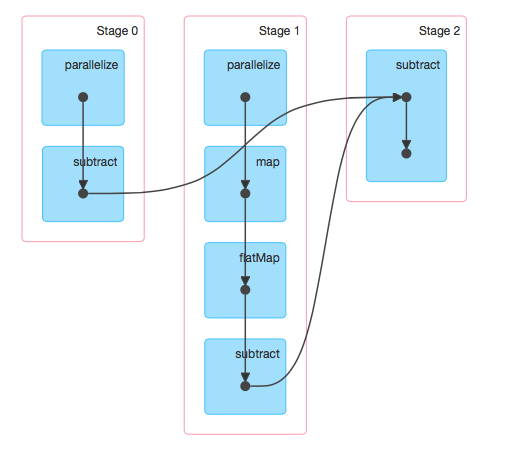
\includegraphics[width=0.8\textwidth]{img/sparkdag.png}
    \caption{Esempio di Spark DAG}
    \label{fig:spark_dag}
\end{figure}


\subsection{Spark Core}
Spark Core è la base dell'intero progetto: fornisce il dispacciamento distribuito dei compiti, lo scheduling e le funzionalità I/O di base. Spark Core funziona in parte come un livello API. Oltre al motore Spark Core, l’ambiente API Apache Spark viene fornito insieme ad alcune librerie da utilizzare nelle applicazioni di analisi dei dati.
\begin{itemize}
    \item \textbf{Spark SQL}: è un modulo Spark per l'elaborazione di dati strutturati. A differenza delle API di base di Spark RDD, le interfacce fornite da Spark SQL forniscono a Spark più informazioni sulla struttura dei dati e sul calcolo che viene eseguito. Internamente, Spark SQL utilizza queste informazioni extra per eseguire ottimizzazioni. Dato che quando si calcola un risultato, viene utilizzato lo stesso motore di esecuzione, indipendentemente da quale API/linguaggio si sta utilizzando, gli sviluppatori possono facilmente fare avanti e indietro tra diverse API a loro piacimento. DataFrame fa parte di questa libreria.
    \item \textbf{Spark Streaming}: una libreria per l'elaborazione scalabile, ad alta velocità e fault-tolerant di flussi di dati in tempo reale.  I dati possono essere ottenuti da molte fonti come Kafka, Kinesis, o socket TCP, possono essere elaborati tramite algoritmi di Machine Learning ed elaborazione grafica ed infine possono essere inviati a file system, database e dashboard live.
    \item \textbf{MLlib}: una libreria di Machine Learning (ML) il cui scopo è di rendere l'apprendimento automatico facile e scalabile. Essa mette a disposizione algoritmi di Machine Learning, Pipelines e diversi altri strumenti per lo svolgimento di operazioni statistiche avanzate sui dati e per creare applicazioni attorno a queste analisi.
    \item \textbf{GraphX}: è un nuovo componente di Spark per i grafi e il calcolo parallelo su di essi. Per supportare il calcolo dei grafi, GraphX mette a disposizione un insieme di operazioni fondamentali (ad esempio, \textit{subgraph}, \textit{joinVertices}, e \textit{aggregateMessages}). Inoltre, include una crescente collezione di algoritmi e costruttori di grafi per semplificare i compiti di analisi.
\end{itemize}

\begin{figure}[hbt!]
    \centering
    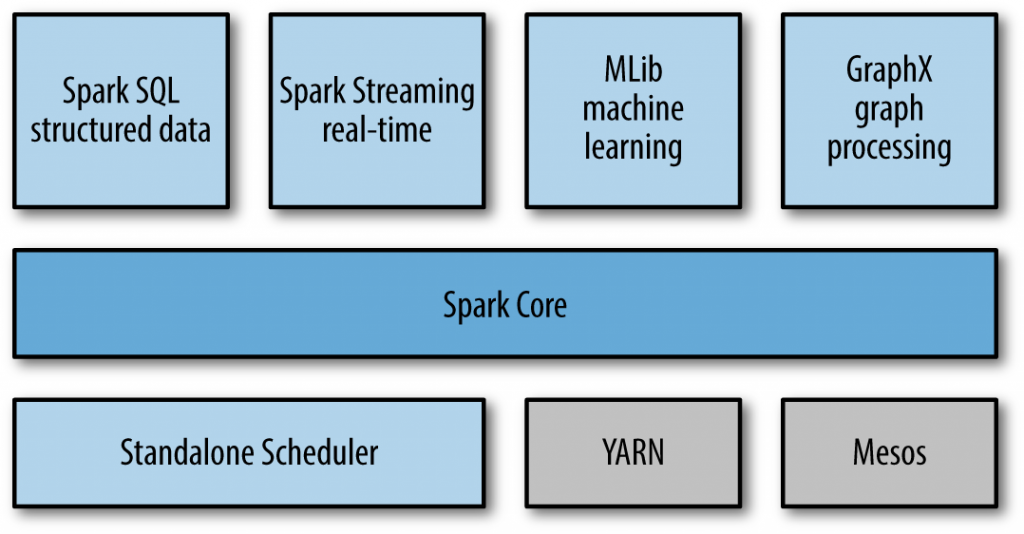
\includegraphics[width=1\textwidth]{img/sparkcore.png}
    \caption{Spark core e librerie}
    \label{fig:spark_core}
\end{figure}
\newpage




\section{Spark NLP}
La popolarità del Natural Language Processing ha fatto si che, negli ultimi anni, siano state sviluppate decine di librerie che risolvono numerosi problemi legati all'argomento (NLTK, SpaCy, Stanford Core NLP e molte altre). In particolare, negli ultimi anni ha attirato particolarmente l'attenzione Spark NLP\footnote{Spark NLP: \href{https://nlp.johnsnowlabs.com/}{https://nlp.johnsnowlabs.com/}}, libreria costruita su Apache Spark e Spark ML. Spark NLP, nata nell'ottobre del 2017 dal \textit{John Snow Labs}, è al momento la soluzione adottata maggiormente dalle aziende, grazie soprattutto alle caratteristiche ereditate da Spark che fanno si che essa ottenga i risultati migliori a livello di accuratezza e velocità di esecuzione su numerosissimi task NLP. Proprio per questo motivo, in questa Tesi, si sono volute testare in prima persona le potenzialità di questo framework.
\subsection{Cosa è Spark NLP}
Spark NLP è una libreria di elaborazione del linguaggio naturale open source, costruita su Apache Spark e Spark ML. Fornisce un’API semplice da integrare con ML Pipelines ed è commercialmente supportato da John Snow Labs.  Gli annotatori di Spark NLP utilizzano algoritmi basati su regole, Machine Learning e Deep Learning. La libreria Spark NLP è scritta in Scala e include API Scala, Java e Python per l’uso da Spark. Copre quasi la totalità dei task NLP comuni, tra cui tokenizzazione, lemmatizzazione, part-of-speech tagging, analisi del sentimento, controllo ortografico e altro ancora attraverso numerosi componenti che raggiungono lo stato dell'arte nella maggior parte dei compiti citati. In particolare, come già citato, in questo progetto sono stati trattati, utilizzando questa libreria, Named Entity Recognition e Text Classification. 

Spark NLP possiede oltre 70 pipelines ed oltre 90 modelli pre-addestrati\footnote{Models Hub: \href{https://nlp.johnsnowlabs.com/models}{https://nlp.johnsnowlabs.com/models}}, sebbene servano da modo per avere un’idea del funzionamento della libreria e non per l’uso in produzione. Essendo un'estensione nativa di Spark ML API, la libreria offre la possibilità di allenare, personalizzare e salvare i modelli in modo che possano essere eseguiti su un cluster, su altre macchine o salvati per un secondo momento (transfer learning).
\subsection{Come funziona Spark NLP}
Spark ML fornisce un insieme di applicazioni di Machine Learning che possono essere costruite
utilizzando due componenti principali: \textbf{Estimators} e \textbf{Trasformers}. Gli Estimators hanno un metodo chiamato \verb|fit(data)| che addestra un pezzo di dati a tale applicazione. Il Transformer\footnote{Elenco Transformers: \href{https://nlp.johnsnowlabs.com/docs/en/transformers}{https://nlp.johnsnowlabs.com/docs/en/transformers}} è generalmente il risultato di un processo di addestramento e applica le modifiche al set di dati di
destinazione. Questi componenti sono stati incorporati per essere applicabili a Spark NLP. Per combinare più estimators e trasformers in un unico flusso di lavoro viene utilizzato il meccanismo delle \textit{Pipelines}. Esse permettono più trasformazioni concatenate lungo un task di Machine Learning restituendo come risultato un'\textbf{annotazione}.

Gli annotatori\footnote{Elenco annotatori: \href{https://nlp.johnsnowlabs.com/docs/en/annotators}{https://nlp.johnsnowlabs.com/docs/en/annotators}} sono la punta di diamante delle funzioni NLP in Spark NLP e sono disponibili in due forme:
\begin{itemize}
    \item \textbf{Annotator Approaches}: sono quelli che rappresentano uno Spark ML Estimator e richiedono una fase di allenamento. Hanno una funzione chiamata \verb|fit(data)| che allena un modello basato su alcuni dati. Producono il secondo tipo di annotatore che è un modello annotatore o trasformatore.
    \item \textbf{Annotator Models}: sono modelli spark o trasformatori, cioè hanno una funzione \textit{transform(data)}. Questa funzione prende come input un dataframe al quale aggiunge una nuova colonna contenente il risultato dell'annotazione corrente. Tutti i trasformatori sono additivi, il che significa che aggiungono ai dati correnti, senza mai sostituire o cancellare le informazioni precedenti
\end{itemize}
Entrambe le forme di annotatori possono essere incluse in una Pipeline. Tutti gli annotatori inclusi in una Pipeline saranno automaticamente eseguiti nell'ordine definito e trasformeranno i dati di conseguenza. Una Pipeline viene trasformata in un \textbf{PipelineModel} dopo la fase \verb|fit(data)|. La Pipeline può essere salvata su disco e ricaricata in qualsiasi momento.

Nel capitolo \ref{sperimentazione} verrà illustrato nel dettaglio come questo framework è stato utilizzato durante la fase di sperimentazione.
\subsection{Perchè usare Spark NLP}
Quali sono quindi i punti di forza di Spark NLP?
\begin{enumerate}
    \item \textbf{Accuratezza}: La libreria Spark NLP 2.0 ha ottenuto i migliori risultati accademici peer-reviewed.
    \item \textbf{Velocità}: Le ragioni della sua velocità sono il motore Tungsten di seconda generazione per i dati colonnari vettoriali in-memoria, nessuna copia del testo in memoria, ampia profilazione, configurazione e ottimizzazione del codice di Spark e TensorFlow, e ottimizzazione per l'addestramento e l'inferenza.
    \item \textbf{Scalabilità}: Questa libreria è capace di scalare allenamento dei modelli, inferenza e pipelines da una macchina locale ad un cluster con piccoli, se non nessun, cambiamenti di codice.
    \item \textbf{Performance}: Spark NLP include caratteristiche che forniscono API Java, Scala e Python complete, supporta la formazione su GPU, supporta reti di deep learning definite dall'utente, supporta Spark nativamente, supporta Hadoop (YARN e HDFS).
    \item \textbf{API in Python, Java e Scala}: Una libreria che supporta più lingue non solo guadagna pubblico, ma permette anche di sfruttare i modelli implementati senza dover spostare i dati avanti e indietro tra gli ambienti di runtime.
\end{enumerate}

\clearpage
\section{Configurazione dell’architettura utilizzata}
Il processo di sperimentazione è stato svolto grazie all'utilizzo di macchine messe a disposizione da \textit{Reveal s.r.l}.
Il codice prodotto è stato prima eseguito su di un PC desktop domestico, per poi essere testato su un piccolo cluster di \clustersize{} macchine. Su di esse sono stati configurati ed installati l'ambiente Apache Spark, Spark NLP e Hadoop. Per testare la scalabilità offerta dal framework del John Snow Labs, il software è stato eseguito prima utilizzando soltanto una macchina per poi incrementare la potenza di calcolo a disposizione migrando l'esecuzione su di un sistema distribuito. 

\subsection{Hardware}
Le configurazioni delle macchine utilizzate sono le seguenti:\\
Configurazione macchina domestica:
\begin{itemize}
    \item Sistema operativo: Windows 10 Home
    \item Numero di CPU: 16
    \item Dimensione RAM: 16GB
\end{itemize}
Configurazione cluster (1 master, 2 workers):
\begin{itemize}
    \item Sistema operativo: CentOS 7
    \item Numero CPU per driver: 8
    \item Dimensione memoria per driver: 10 GB
    \item Numero di CPU per ogni worker: 4
    \item Dimensione memoria per ogni worker: 10 GB
\end{itemize}

\subsection{Software}
Come citato precedentemente, l'obiettivo è quello di testare soluzioni per la risoluzione di task di NLP in ambiente distribuito, confrontando i risultati ottenuti in termini di accuratezza e tempi di esecuzione. Per eseguire l'applicazione, all'interno del sistema sono stati configurati: l'ambiente Spark, un database distribuito HDFS ed il resource manager YARN. 

Nella macchina master risiedono il driver di Spark, il \textbf{NameNode} (deamon per HDFS), responsabile della gestione del namespace del file system e il \textbf{ResourceManager} (deamon per YARN), responsabile dell’assegnazione e della gestione delle risorse tra tutte le applicazioni. Quando Spark NLP richiede al sistema l'esecuzione di un job o di un DAG di jobs, questa richiesta viene inoltrata all'istanza di YARN in esecuzione sul nodo master che verifica se l'esecuzione è possibile e, in caso affermativo, registra l'applicazione assegnandogli un Job ID e aggiungendolo alla coda dei job da eseguire. 

Ogni volta che un job viene estratto dalla coda ed è mandato in esecuzione, il ResourceManager seleziona casualmente un DataNode (processo di HDFS) e avvia su quello stesso nodo un processo ApplicationMaster (processo di YARN). Al passo successivo, l'ApplicationMaster comunicherà con il NameNode che a sua volta si occuperà di accertarsi della posizione in cui si trovano i file (blocchi) all'interno del cluster e di quante risorse ha bisogno il job. 

Una volta svolte tutte le valutazioni, l'ApplicationMaster invia le informazioni sulla richiesta di risorse al ResourceManager che le esamina e inoltra una richiesta di allocazione di queste, sotto forma di container, ai nodi del cluster. Questi container sono detti \textit{Esecutori}. I NodeManager di ogni singolo nodo worker si occuperanno quindi di allocare le risorse come da richiesta del ResourceManager. 

Infine, gli esecutori inizieranno l'esecuzione dei job a loro assegnati e proseguiranno la comunicazione direttamente con il programma driver (SparkContext). L'output sarà direttamente restituito al client.

Sul cluster utilizzato in questo progetto, l'applicazione è stata eseguita nella cosiddetta \textit{Client Mode}, ovvero, il driver Spark viene avviato sulla stessa macchina da cui viene inviata l'applicazione.

\begin{figure}[hbt!]
    \centering
    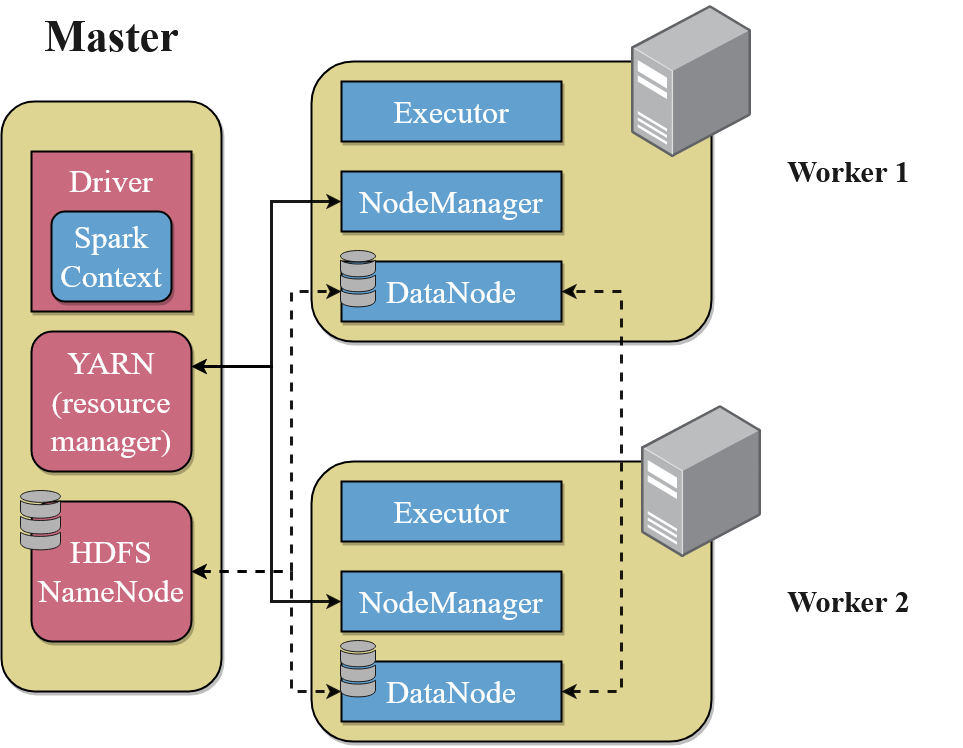
\includegraphics[width=1\textwidth]{img/architecture/cluster_architecture2.png}
    \caption{Architettura del cluster}
    \label{fig:cluster_architecture}
\end{figure}

\begin{figure}[hbt!]
    \centering
    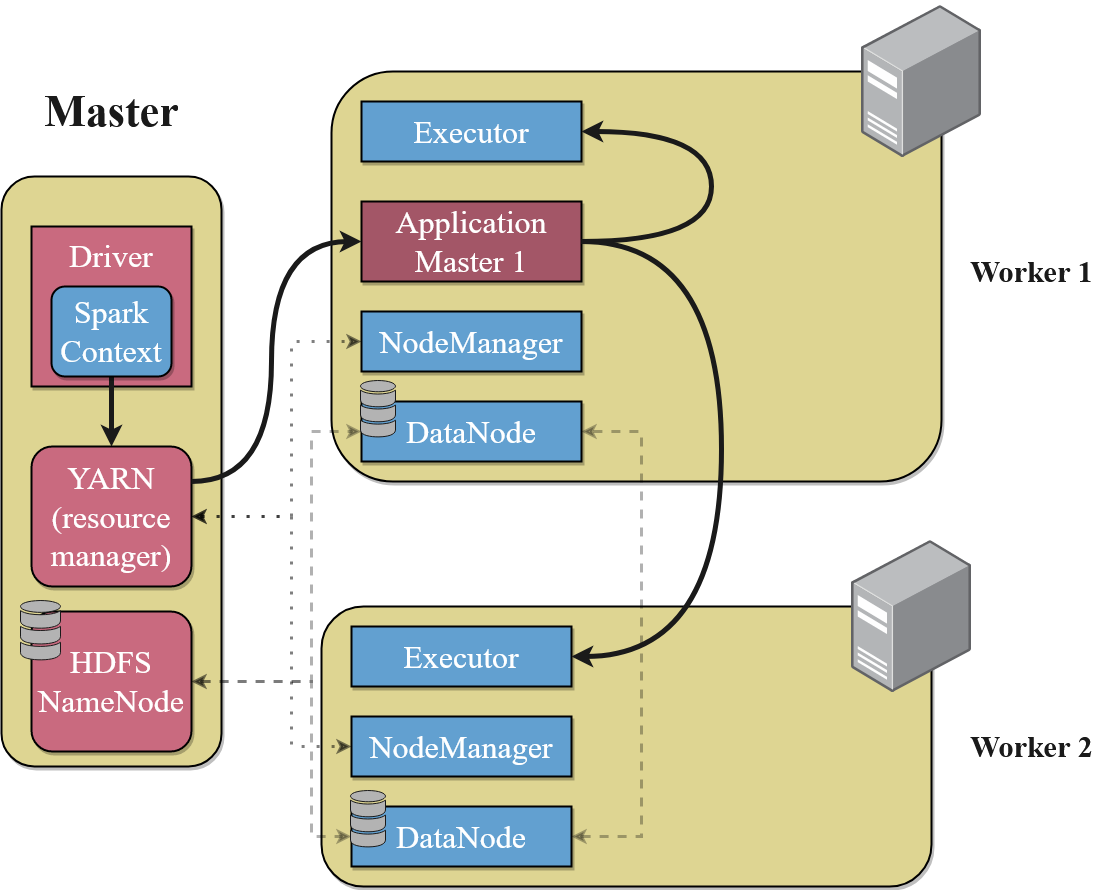
\includegraphics[width=0.7\textwidth]{img/architecture/application_submit2.png}
    \caption{Richiesta di esecuzione dell'applicazione}
    \label{fig:application_submit}
\end{figure}

\begin{figure}[hbt!]
    \centering
    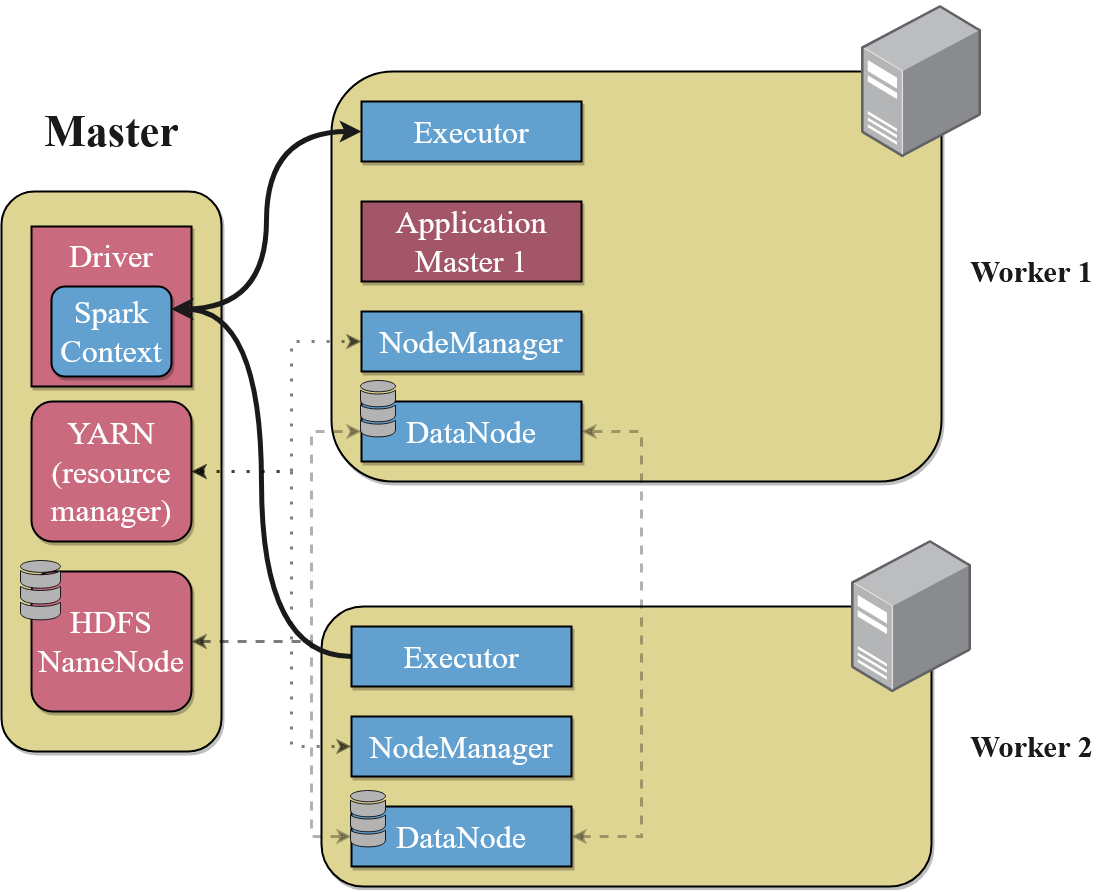
\includegraphics[width=0.7\textwidth]{img/architecture/jobs_execution2.png}
    \caption{Esecuzione dei compiti: interazione tra esecutori e driver}
    \label{fig:jobs_execution}
\end{figure}


\chapter{Sperimentazione}  \label{sperimentazione}
%cappello introduttivo
In questo capitolo verrà trattata nel dettaglio la fase di sperimentazione dalla quale nasce questa Tesi. Verranno trattati i task che il software prodotto tenta di risolvere e come sono state introdotte ed utilizzate le tecnologie descritte nel capitolo \ref{sol_distribuita}. Infine seguirà un'analisi dei risultati ottenuti.
%sezioni
\section{Text Classification}
%cappello introduttivo
In questa sezione verrà trattato il task di \textit{Text Classification} e verrà illustrato il dataset utilizzato. 
%sezioni
\subsection{Descrizione del task}
La \textbf{classificazione del testo}, conosciuta anche come \textit{tagging del testo} o \textit{categorizzazione del testo}, è il processo di categorizzazione dei corpora in gruppi organizzati. Utilizzando il Natural Language Processing, i classificatori possono analizzare automaticamente i testi e poi assegnare loro un insieme di tag o categorie predefinite in base al suo contenuto. \citet{textclassificationproblem_stanford}, ricercatori della Stanford University, definiscono il problema nella maniera seguente. 

Nella classificazione del testo, ci viene data una descrizione \(d\in \mathbb{X}\) di un documento, dove \(\mathbb{X}\) è lo \textit{spazio dei documenti}, e un insieme fissato di \textit{classi} \(\mathbb{C}={c_1,c_2,...,c_j}\), chiamate anche \textit{categorie} o \textit{etichette}. Tipicamente, lo spazio dei documenti \(\mathbb{X}\) è un qualche tipo di spazio di grandi dimensioni (high-dimensional space), e le classi sono definite dall'uomo per la necessità di una specifica applicazione. Ci viene fornito anche un insieme per l'addestramento \(\mathbb{D}\) di documenti etichettati \(\langle d,c \rangle \in \mathbb{X} \times \mathbb{C}\).
Per esempio:
\begin{center}
\(\langle d,c \rangle\) = \(\langle\) Pechino entra nell'Organizzazione Mondiale del Commercio, China \(\rangle\)
\end{center}
per il documento \textit{Pechino entra nell'Organizzazione Mondiale del Commercio} e la classe \textit{China}.

Utilizzando un \textit{algoritmo di apprendimento}, vogliamo poi creare un classificatore o una \textit{funzione di classificazione} \(\gamma\) che mappa documenti in classi:
\begin{center}
\(\gamma:\mathbb{X}\rightarrow\mathbb{C}\)
\end{center}

Questo tipo di apprendimento è chiamato \textbf{apprendimento supervisionato} perché un supervisore (la persona che definisce le classi ed etichetta i documenti utilizzati per l'addestramento) serve come un \textit{insegnante} che dirige il processo di apprendimento. Per il momento, consideriamo solo i problemi \textit{one-of} in cui un documento è membro esattamente di una classe: il nostro obiettivo nella classificazione del testo è un'alta accuratezza sui dati di test. 

La classificazione del testo sta diventando una parte sempre più importante nelle aziende, poiché permette di ottenere facilmente informazioni dai dati e automatizzare i processi aziendali. Alcuni degli esempi e dei casi d'uso più comuni per la classificazione automatica del testo sono i seguenti:

\begin{itemize}
    \item \textbf{Sentiment Analysis}: il processo di capire se un dato testo sta parlando positivamente o negativamente di un dato argomento (ad esempio per scopi di monitoraggio del marchio).
    \item \textbf{Language Detection}: la procedura di rilevamento della lingua di un dato testo (ad esempio sapere se un ticket di supporto in arrivo è scritto in inglese o in spagnolo per indirizzarlo automaticamente al team appropriato).
    \item \textbf{Topic Detection}: il compito di identificare il tema o l'argomento di una porzione di testo (ad esempio, sapere se una recensione di un prodotto da parte di un cliente riguarda la facilità d'uso, il supporto clienti o il prezzo). Questo è il compito che è stato studiato durante la fase di analisi descritta in questo capitolo.
\end{itemize}

\begin{figure}[hbt!]
    \centering
    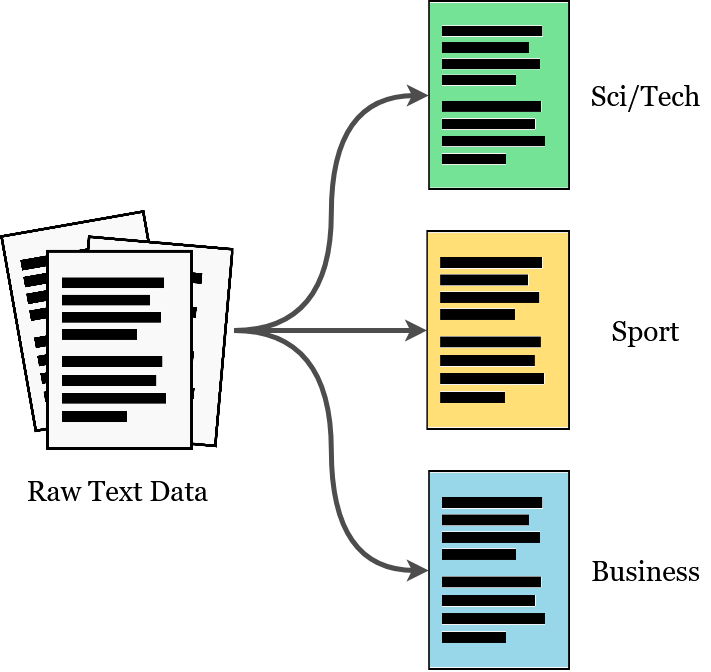
\includegraphics[width=0.5\textwidth]{img/textc_example.png}
    \caption{Text Classification: topic detection}
    \label{fig:textc_example}
\end{figure}
\subsection{Il dataset} \label{textc_data}
Il dataset utilizzato è stato messo a disposizione dagli sviluppatori di SparkNLP (John Snow Lab) per un workshop da loro svolto e reso disponibile sul loro profilo Github\footnote{Repository: \href{https://github.com/JohnSnowLabs/spark-nlp-workshop/tree/master/tutorials/Certification_Trainings/Public/data}{https://github.com/JohnSnowLabs/spark-nlp-workshop/}}. 

Il dataset è composto da due file: \textit{news\_category\_train.csv} con 120.000 esempi per l’addestramento e \textit{news\_category\_test.csv} con 7.600 esempi per il testing.
Ogni riga di entrambi i file è formata dai campi \textbf{description} e \textbf{category}. Il primo contiene il testo da classificare, il secondo indica di quale categoria fa parte il testo. Ogni testo appartiene esattamente ad una sola classe.
In totale, ci sono 4 categorie: \textit{Business}, \textit{Sci/Tech}, \textit{World}, \textit{Sports}.\\
\begin{figure}[hbt!]
    \centering
    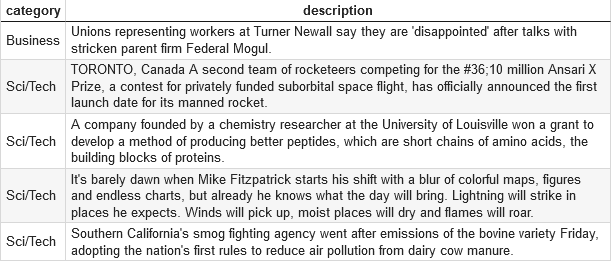
\includegraphics[width=0.9\textwidth]{img/textc_dataset.png}
    \caption{Porzione del dataset per Text Classification}
    \label{fig:textc_dataset}
\end{figure}
\subsection{Spark NLP per Text Classification}
Spark NLP dispone di un annotatore chiamato \textit{ClassifierDL}, un classificatore multi-classe che utilizza una Deep Neural Network e supporta fino a 100 classi diverse. ClassifierDL richiede dei \verb|SENTENCE_EMBEDDINGS| (ovvero embedding di intere frasi) come input e restituisce una predizione sulla categoria a cui appartiene il testo.

I dataset estratti dai file in formato \verb|CSV| (descritti nel paragrafo \ref{textc_data}) vengono importati in uno \verb|Spark Dataframe| (argomento trattato nel paragrafo \ref{rdd_df}).

Per ottenere gli embeddings a partire dal testo, Spark NLP mette a dispozione diverse alternative; i due componenti utilizzati in questo progetto sono:
\begin{itemize}
    \item \textbf{Universal Sentence Encoder}
    \item \textbf{Bert Sentence Embeddings}
\end{itemize}
Non è il nostro scopo studiare come avviene l’addestramento dei modelli utilizzati per la produzione degli embeddings, pertanto verrano utilizzati modelli pre-addestrati presenti nella sezione 
\textit{NLP Models Hub}\footnote{Models Hub: \href{https://nlp.johnsnowlabs.com/models}{https://nlp.johnsnowlabs.com/models}} 
della documentazione di Spark NLP. Per la precisione sono stati importati:
\begin{itemize}
    \item \verb|tfhub_use|\footnote{tfhub\_use: \href{https://nlp.johnsnowlabs.com/2020/04/17/tfhub\_use.html}{https://nlp.johnsnowlabs.com/2020/04/17/tfhub\_use.html}} per \verb|UniversalSentenceEncoder|, addestrato con una Deep Averaging Network (DAN)
    \item \verb|sent_bert_base_cased|\footnote{sent\_bert\_base\_cased\href{https://nlp.johnsnowlabs.com/2020/08/25/sent\_bert\_base\_cased.html}{https://nlp.johnsnowlabs.com/2020/08/25/sent\_bert\_base\_cased.html}} per \verb|BertSentenceEmbeddings| (24 Layers di dimensione 1024).
\end{itemize}
Le \textit{pipelines} sono costruite seguendo il seguente ordine:
\begin{enumerate}
    \item \verb|Document Assembler|: prepara i dati in un formato processabile da Spark NLP.
    \item \verb|Encoder| (USE o Bert Sentence Embeddings): aggiunge una colonna al Dataframe dove, per ogni riga viene aggiunto il vettore ottenuto codificando il testo.
    \item \verb|ClassifierDL|: data in input la colonna degli embeddings ottenuta dallo step precedente, si occupa della classificazione ed aggiunge un'ulteriore colonna nella quale viene inserita la predizione della classe associata al testo.
\end{enumerate}
\clearpage
\section{Named Entity Recognition}
%cappello introduttivo
In questa sezione verrà trattato il task di \textit{Named Entity Recognition} e verranno illustrati i due dataset utilizzati, rispettivamente in lingua inglese e in lingua italiana. 
%sezioni
\subsection{Descrizione del task}
La \textbf{classificazione del testo}, conosciuta anche come \textit{tagging del testo} o \textit{categorizzazione del testo}, è il processo di categorizzazione dei corpora in gruppi organizzati. Utilizzando il Natural Language Processing, i classificatori possono analizzare automaticamente i testi e poi assegnare loro un insieme di tag o categorie predefinite in base al suo contenuto. \citet{textclassificationproblem_stanford}, ricercatori della Stanford University, definiscono il problema nella maniera seguente. 

Nella classificazione del testo, ci viene data una descrizione \(d\in \mathbb{X}\) di un documento, dove \(\mathbb{X}\) è lo \textit{spazio dei documenti}, e un insieme fissato di \textit{classi} \(\mathbb{C}={c_1,c_2,...,c_j}\), chiamate anche \textit{categorie} o \textit{etichette}. Tipicamente, lo spazio dei documenti \(\mathbb{X}\) è un qualche tipo di spazio di grandi dimensioni (high-dimensional space), e le classi sono definite dall'uomo per la necessità di una specifica applicazione. Ci viene fornito anche un insieme per l'addestramento \(\mathbb{D}\) di documenti etichettati \(\langle d,c \rangle \in \mathbb{X} \times \mathbb{C}\).
Per esempio:
\begin{center}
\(\langle d,c \rangle\) = \(\langle\) Pechino entra nell'Organizzazione Mondiale del Commercio, China \(\rangle\)
\end{center}
per il documento \textit{Pechino entra nell'Organizzazione Mondiale del Commercio} e la classe \textit{China}.

Utilizzando un \textit{algoritmo di apprendimento}, vogliamo poi creare un classificatore o una \textit{funzione di classificazione} \(\gamma\) che mappa documenti in classi:
\begin{center}
\(\gamma:\mathbb{X}\rightarrow\mathbb{C}\)
\end{center}

Questo tipo di apprendimento è chiamato \textbf{apprendimento supervisionato} perché un supervisore (la persona che definisce le classi ed etichetta i documenti utilizzati per l'addestramento) serve come un \textit{insegnante} che dirige il processo di apprendimento. Per il momento, consideriamo solo i problemi \textit{one-of} in cui un documento è membro esattamente di una classe: il nostro obiettivo nella classificazione del testo è un'alta accuratezza sui dati di test. 

La classificazione del testo sta diventando una parte sempre più importante nelle aziende, poiché permette di ottenere facilmente informazioni dai dati e automatizzare i processi aziendali. Alcuni degli esempi e dei casi d'uso più comuni per la classificazione automatica del testo sono i seguenti:

\begin{itemize}
    \item \textbf{Sentiment Analysis}: il processo di capire se un dato testo sta parlando positivamente o negativamente di un dato argomento (ad esempio per scopi di monitoraggio del marchio).
    \item \textbf{Language Detection}: la procedura di rilevamento della lingua di un dato testo (ad esempio sapere se un ticket di supporto in arrivo è scritto in inglese o in spagnolo per indirizzarlo automaticamente al team appropriato).
    \item \textbf{Topic Detection}: il compito di identificare il tema o l'argomento di una porzione di testo (ad esempio, sapere se una recensione di un prodotto da parte di un cliente riguarda la facilità d'uso, il supporto clienti o il prezzo). Questo è il compito che è stato studiato durante la fase di analisi descritta in questo capitolo.
\end{itemize}

\begin{figure}[hbt!]
    \centering
    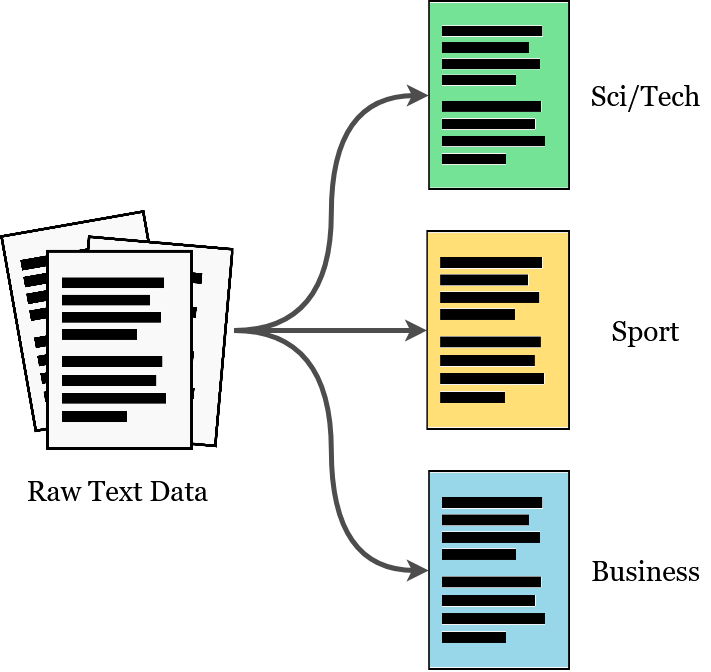
\includegraphics[width=0.5\textwidth]{img/textc_example.png}
    \caption{Text Classification: topic detection}
    \label{fig:textc_example}
\end{figure}
\subsection{Dataset in lingua inglese} \label{ner_eng_data}
\label{sec:ner_dataset_en}
Il dataset utilizzato è la versione in inglese del task CoNLL-2003, disponibile nella repository Github\footnote{Dataset: \href{https://github.com/JohnSnowLabs/spark-nlp/tree/master/src/test/resources/conll2003}{https://github.com/JohnSnowLabs/spark-nlp/tree/master/src/test/resources/conll2003}} di Spark NLP. 

Il dataset è composto da tre file: \textit{eng.train} con 14.041 esempi per l’addestramento, \textit{eng.test} con 6.603 esempi per il testing.

Il primo elemento su ogni riga è una parola, il secondo un tag \textbf{part-of-speech (POS)}, il terzo un tag \textbf{chunk sintattico} e il quarto il tag \textbf{named entity}. I tag chunk e i tag named entity hanno il formato \textit{I-TYPE} che significa che la parola è dentro una frase di tipo \textit{TYPE}. Solo se due frasi dello stesso tipo si susseguono immediatamente, la prima parola della seconda frase avrà il tag \textit{B-TYPE} per mostrare che inizia una nuova frase. Una parola con il tag \textit{O} non fa parte di una frase. Le entità presenti nel dataset sono: \textit{persone}, \textit{luoghi}, \textit{organizzazioni} ed entità \textit{varie} che non appartengono ai tre gruppi precedenti.
\begin{figure}[hbt!]
    \centering
    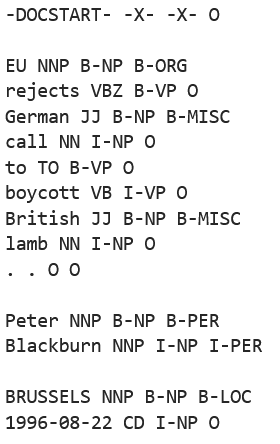
\includegraphics[width=0.25\textwidth]{img/ner_en_dataset.png}
    \caption{Porzione del dataset per NER in lingua inglese}
    \label{fig:ner_en_dataset}
\end{figure}

\subsection{Dataset in lingua italiana} \label{ner_ita_data}
\label{sec:ner_dataset_it}
Il dataset utilizzato per l'italiano è stato generato utilizzando training e test set di Named Entity Recognition di EVALITA 2009\footnote{Evalita 2009: \href{https://www.evalita.it/evalita-2009/tasks/entity-recognition/}{https://www.evalita.it/evalita-2009/tasks/entity-recognition/}}. La valutazione è basata sull' \textit{Italian Content Annotation Bank} (I-CAB) dove le entità nominate sono annotate nel formato \textit{IOB} (dove "B-begin" e "I-inside" denotano i token appartenenti a Named Entities e "O-outside" è usato per tutti gli altri token). Per la precisione sono state rigenerate le quattro colonne presenti anche nel dataset in lingua inglese (vedi pagina \pageref{sec:ner_dataset_en}):
\begin{enumerate}
    \item La prima colonna contiene ogni \textbf{token} iniziale della frase.
    \item La seconda il \textbf{POS tag}, secondo il tagset ISST-TANL\footnote{ISST-TANL: \href{http://www.italianlp.it/docs/ISST-TANL-POStagset.pdf}{http://www.italianlp.it/docs/ISST-TANL-POStagset.pdf}}.
    \item  La terza colonna NON contiene il \textbf{chunk sintattico}, che non era previsto nella competizione. Per simmetria con il dataset inglese è stata aggiunta la colonna, ma ogni riga contiene solo il token "\_".
    \item La quarta colonna racchiude il tag della \textbf{named entity} che rispecchia la descrizione del sito, riportata anche sopra.
\end{enumerate}
Il dataset è composto da due file: \textit{I-CAB-evalita09-NER-train\_utf8.tsv} con 11.227 esempi per l’addestramento e \textit{I-CAB-evalita09-NER-test\_utf8.tsv} con 4.136 esempi per il testing.

Le entità presenti nel dataset sono: \textit{persone}, \textit{luoghi}, \textit{organizzazioni} ed entità \textit{geo-politiche}.
\begin{figure}[hbt!]
    \centering
    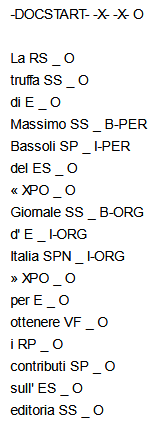
\includegraphics[width=0.17\textwidth]{img/ner_it_dataset.png}
    \caption{Porzione del dataset per NER in lingua italiana}
    \label{fig:ner_it_dataset}
\end{figure}


\section{Spark NLP}
La popolarità del Natural Language Processing ha fatto si che, negli ultimi anni, siano state sviluppate decine di librerie che risolvono numerosi problemi legati all'argomento (NLTK, SpaCy, Stanford Core NLP e molte altre). In particolare, negli ultimi anni ha attirato particolarmente l'attenzione Spark NLP\footnote{Spark NLP: \href{https://nlp.johnsnowlabs.com/}{https://nlp.johnsnowlabs.com/}}, libreria costruita su Apache Spark e Spark ML. Spark NLP, nata nell'ottobre del 2017 dal \textit{John Snow Labs}, è al momento la soluzione adottata maggiormente dalle aziende, grazie soprattutto alle caratteristiche ereditate da Spark che fanno si che essa ottenga i risultati migliori a livello di accuratezza e velocità di esecuzione su numerosissimi task NLP. Proprio per questo motivo, in questa Tesi, si sono volute testare in prima persona le potenzialità di questo framework.
\input{Capitoli_Interni/Capitolo3/Sottosezioni_4/1_SparkNLPIntro}
\input{Capitoli_Interni/Capitolo3/Sottosezioni_4/2_Funzionamento}
\input{Capitoli_Interni/Capitolo3/Sottosezioni_4/3_UsareSparkNLP}

\clearpage
\newpage
\subsection{Tabelle riassuntive dataset}

\subsubsection{Text Classification}
\begin{table}[ht!]
    \centering
    \begin{tabular}{|c|c|c|}
        \hline
            \textbf{Utilizzo} & \textbf{Formato} & \textbf{Numero di esempi} \\
        \hline
            Addestramento & CSV & 120.000\\
        \hline
            Test & CSV & 7.600 \\
        \hline
    \end{tabular}
    \caption{Dataset per Text Classification}
    \label{tab:dataset_textc}
\end{table}

\subsubsection{Named Entity Recognition}
\begin{table}[ht!]
    \centering
    \begin{tabular}{|c|c|c|c|}
        \hline
            \textbf{Lingua} & \textbf{Utilizzo} & \textbf{Formato} & \textbf{Numero di esempi} \\
        \hline
            \multirow{2}*{Inglese} & Addestramento  & CoNLL '03 & 14.041     \\
            \cline{2-4}            & Test & CoNLL '03 & 6.603    \\
        \hline
            \multirow{2}*{Italiano} & Addestramento  & CoNLL '03 & 11.227     \\
            \cline{2-4}            & Test & CoNLL '03 & 4.136    \\
        \hline
    \end{tabular}
    \caption{Dataset per NER}
    \label{tab:dataset_ner}
\end{table}
\newpage
\section{Analisi Prestazionale}
Costruite le pipelines, a partire da ognuna di esse è stato addestrato un modello utilizzando il metodo \verb|.fit()|:
\begin{center}
    \verb|pipelineModel = pipeline.fit(train_data)|
\end{center}
Una volta pronto il modello, è stato testato utilizzando il metodo \verb|.transform()|. Facendo ciò, viene generato un nuovo DataFrame aggiungendo a quello di partenza una colonna con le previsioni fatte dal modello:
\begin{center}
    \verb|predictions = pipelineModel.transform(test_data)|
\end{center}
Utilizzando i modelli addestrati, sono state svolte due tipi di valutazioni. La prima tiene conto dell'accuratezza delle predizioni ottenute dai modelli utilizzando i dataset di test descritti nelle sezioni \ref{textc_data}, \ref{ner_eng_data} e \ref{ner_ita_data}. La seconda misura i tempi di esecuzione ottenuti parallelizzando il lavoro ed opera su di un dataset di 760.000 record.
\subsection{Metriche} \label{metriche}
A partire dalle previsioni prodotte, è stato generato un \textit{classification report}. Si tratta di un rapporto che descrive varie metriche relative a quanto bene ha funzionato un modello di machine learning e che si ottengono confrontando i risultati prodotti dal modello con quelli attesi. Il report mostra le principali metriche di classificazione:
\begin{itemize}
    \item \textbf{Precisione (Precision)}: la capacità di un classificatore di identificare solo le istanze corrette per ogni classe.
    \item \textbf{Richiamo (Recall)}: la capacità di un classificatore di trovare tutte le istanze corrette per una classe.
    \item \textbf{F1-Score}: media armonica ponderata di precisione e richiamo normalizzata tra 0 e 1. Un punteggio F di 1 indica un equilibrio perfetto, poiché precisione e richiamo sono inversamente correlati.
    \item \textbf{Accuratezza (Accuracy)}: valore che indica quanto spesso ci si può aspettare che il modello di machine learning preveda correttamente un risultato sul numero totale di volte che ha fatto previsioni.
    \item \textbf{Support}: numero di occorrenze effettive di una classe nel dataset.
\end{itemize}
Per i due task sono state utilizzate due tipi di valutazione differenti:
\begin{itemize}
    \item \textbf{Text Classification}: per questo task è stata scelta una valutazione rigida. Per ogni testo presente nel dataset, se la previsione del modello corrisponde al valore atteso, allora viene valutato come corretto, altrimenti come incorretto. Pertanto, il valore a cui si fa riferimento è l'accuratezza, che si calcola come il rapporto tra le predizioni corrette ed il numero di esempi totali.
    
    \item \textbf{Named Entity Recognition}: per il NER, si prende come riferimento la valutazione proposta nel task CoNLL-2003\footnote{CoNLL-2003 Paper: \href{https://aclanthology.org/W03-0419.pdf}{https://aclanthology.org/W03-0419.pdf}} e nello script \textit{conlevall}\footnote{conlleval script in perl: \href{https://www.clips.uantwerpen.be/conll2000/chunking/conlleval.txt}{https://www.clips.uantwerpen.be/conll2000/chunking/conlleval.txt}}.Le prestazioni dei sistemi sono misurate in termini di precisione, richiamo e f1-score, dove:\\
    \textit{"La precisione è la percentuale di named entities trovate dal sistema di apprendimento che sono corrette. Recall è la percentuale di entità presenti nel corpus che vengono trovate dal sistema. Una named entity è corretta solo se c'è una corrispondenza esatta dell'entità corrispondente nel file di dati".}\\
    Pertanto, il calcolo non tiene in considerazione le previsioni del tag \textit{'O'} (ovvero, chunk che non è una named entity) che sono invece valutate dall'accuracy.
\end{itemize}
\newpage
\subsection{Performance}
\renewcommand{\arraystretch}{2}
% -----------------
%  Text Classification - Inglese
% -----------------
\subsubsection{Text Classification - Inglese}
\begin{table}[hbt!]
    \centering
    \begin{tabular}{|c|c|}
      \hline
          Embedding & Accuracy  \\
      \hline
             USE    &   89\%    \\
      \hline
        Sentence BERT (base\_case)    &   89\%   \\
      \hline
    \end{tabular}
    
    \caption{Risultati per Text Classification}
    \label{tab:textc_results}
\end{table}

\begin{figure}[ht!]
    \centering
    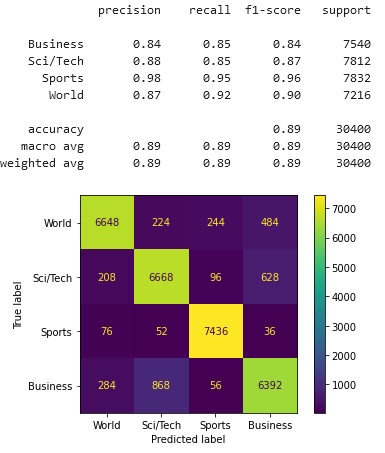
\includegraphics[width=0.7\textwidth]{img/results/cmatrix_textc_use.png}
    \caption{Text Classification - USE: classification report}
    \label{fig:creport_textc_use}
\end{figure}
\begin{figure}[ht!]
    \centering
    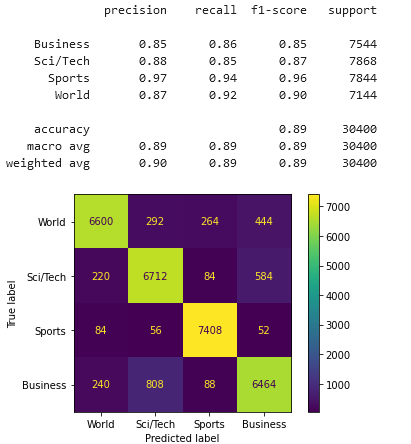
\includegraphics[width=0.7\textwidth]{img/results/cmatrix_textc_bert.png}
    \caption{Text Classification - BERT: classification report}
    \label{fig:creport_textc_bert}
\end{figure}

% -----------------
%  Named Entity Recognition - Inglese
% -----------------
\clearpage
\subsubsection{Named Entity Recognition - Inglese}
\begin{table}[ht!]
    \centering

    \begin{tabular}{|c|c|}
      \hline
        Embedding & F1-Score \\
      \hline
          GloVe  &   85.8\% \\
      \hline
          BERT (base\_case)   &   86.5\% \\
      \hline
    \end{tabular}
    \caption{Risultati per NER in Inglese}
    \label{tab:ner_eng_results}
\end{table}
\begin{figure}[hbt!]
    \centering
    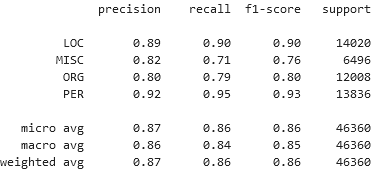
\includegraphics[width=0.7\textwidth]{img/results/creport_ner_eng_glove.png}
    \caption{NER in Inglese - GloVe: classification report}
    \label{fig:creport_ner_eng_glove}
\end{figure}
\begin{figure}[ht!]
    \centering
    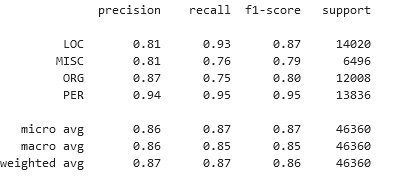
\includegraphics[width=0.7\textwidth]{img/results/creport_ner_eng_bert.png}
    \caption{NER in Inglese - BERT: classification report}
    \label{fig:creport_ner_eng_bert}
\end{figure}

% -----------------
%  Named Entity Recognition - Italiano
% -----------------
\clearpage
\subsubsection{Named Entity Recognition - Italiano}
\begin{table}[hbt!]
    \centering

    \begin{tabular}{|c|c|}
      \hline
        Embedding & F1-Score \\
      \hline
          GloVe  &   65\% \\
      \hline
          BERT (base\_case)  &   60.5\% \\
      \hline
    \end{tabular}
    \caption{Risultati per NER in Inglese}
    \label{tab:ner_ita_results}
\end{table}
\begin{figure}[hbt!]
    \centering
    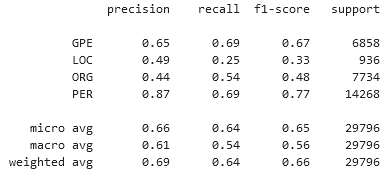
\includegraphics[width=0.7\textwidth]{img/results/creport_ner_ita_glove.png}
    \caption{NER in Italiano - GloVe: classification report}
    \label{fig:creport_ner_ita_glove}
\end{figure}
\begin{figure}[hbt!]
    \centering
    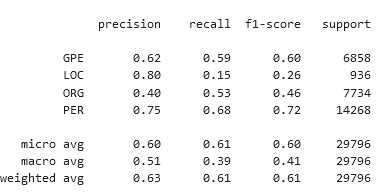
\includegraphics[width=0.7\textwidth]{img/results/creport_ner_ita_bert.png}
    \caption{NER in Italiano - BERT: classification report}
    \label{fig:creport_ner_ita_bert}
\end{figure}
\clearpage
\subsection{Tempi di esecuzione}
\begin{table}[ht!]
    \centering
    \begin{tabular}{|c|c|c|}
        \hline
            Embedding & Esecutori & Tempo di esecuzione     \\
        \hline
            \multirow{2}*{USE} &     1     &  8min 05s      \\
            \cline{2-3}        &     2     &  4min 21s      \\
        \hline
            %\multirow{2}*{Sentence BERT (base\_case)} &     1     &  8h 6min 03s  \\
            \multirow{2}*{BERT (base\_case)} &     1     &  8h 6min 03s  \\
            \cline{2-3}         &     2     &  4h 6min 05s  \\
        \hline
    \end{tabular}
    %\caption{Text Classification - Tempi di esecuzione}
    \caption{Tempi di esecuzione}
    \label{tab:execution_time}
\end{table}

% \begin{table}[ht!]
%     \centering
%     \begin{tabular}{|c|c|c|}
%         \hline
%             Embedding & Esecutori & Tempo di esecuzione     \\
%         \hline
%             \multirow{2}*{GloVe} &     1     &  ???      \\
%             \cline{2-3}          &     2     &  ???      \\
%         \hline
%             \multirow{2}*{BERT} &     1     &  ???  \\
%             \cline{2-3}         &     2     &  ???  \\
%         \hline
%     \end{tabular}
%     \caption{Named Entity Recognition - Tempi di esecuzione}
%     \label{tab:execution_time}
% \end{table}
\subsection{Valutazioni}
Nel caso del task di Named Entity Recognition, i risultati presentano una notevole differenza tra le performance ottenute con i dataset in lingua inglese e in lingua italiana. Infatti, si passa da un F1-score dell'87\% con BERT Base nel primo caso, ad un 60\% con il modello corrispettivo per la lingua italiana. Il risultato per l'inglese non raggiunge lo stato dell'arte\footnote{Risultati CoNLL 2003 (English): \href{https://paperswithcode.com/sota/named-entity-recognition-ner-on-conll-2003}{https://paperswithcode.com/sota/named-entity-recognition-ner-on-conll-2003}}, ma non si distacca eccessivamente dalle altre soluzioni al momento disponibili. Drastico è il calo che si ha con la lingua italiana, dove il modello sbaglia eccessivamente. Da quanto si evince dei risultati mostrati sul sito di \textit{evalita}\footnote{Risultati evalita 2009: \href{https://www.evalita.it/evalita-2009/results/}{https://www.evalita.it/evalita-2009/results/}}, le soluzioni per questo task raggiungono anche valori di F1-score pari all'82\%, ovvero circa il 20\% in più del modello studiato in questa tesi. I risultati peggiori, come si legge dal classification report, si incontrano nei casi dei tag che identificano \textit{entità geo-politiche (GPE)} e \textit{organizzazioni (ORG)}.
\begin{figure}[ht!]
    \centering
    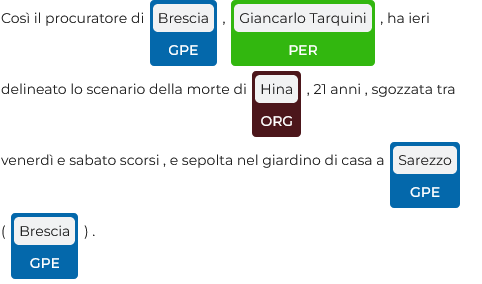
\includegraphics[width=0.8\textwidth]{img/errori_ner_ita/errore1.png}
    \caption{Named Entity Recognition per l'italiano - Errore 1}
    \label{fig:ner_errore1}
\end{figure}
\begin{figure}[ht!]
    \centering
    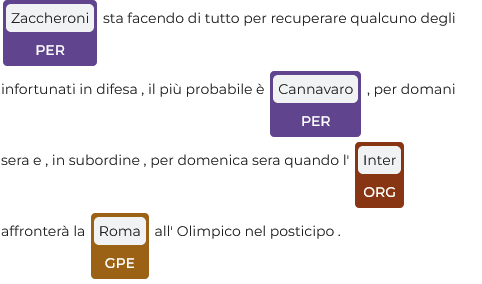
\includegraphics[width=0.8\textwidth]{img/errori_ner_ita/errore2.png}
    \caption{Named Entity Recognition per l'italiano - Errore 2}
    \label{fig:ner_errore2}
\end{figure} \newpage
Osservando la figura \ref{fig:ner_errore1}, si nota come nomi poco frequenti in Italia (in questo caso \textit{Hina}), non vengono interpretati come riferimenti a persone, ma ad altre entità (in questo caso \textit{organizzazione (ORG)}).
Inoltre, il modello fatica a distinguere le ambiguità che si presentano quando un'entità che solitamente è utilizzata con un significato, si presenta nella frase con un'altra accezione. Facendo riferimento all'immagine \ref{fig:ner_errore2}, il concetto di \textit{Roma} come associazione sportiva, e quindi \textit{organizzazione}, viene confuso con il significato di \textit{Roma} intesa come la città capitale d'Italia. La parola è stata pertanto classificata come entità \textit{geo-politica}.
 

Un'ulteriore differenza tra i dati ottenuti dai due dataset, si ha con l'accuratezza raggiunta dai modelli. Anche se di poco, BERT performa meglio di GloVe nella lingua inglese (86.5\% il primo, 85,8\% il secondo), mentre per la lingua italiana, GloVe riconosce leggermente meglio le ambiguità rispetto alla controparte (65\% per GloVe, 60,5\% BERT).\\
\\
Passando al problema di Text Classification, sia il componente UniversalSentenceEncoder sia il BertSentenceEmbedding, riportano ottimi risultati in termini di accuratezza, raggiungendo entrambi l'89\%. La differenza sostanziale si nota nei tempi di esecuzione, nei quali l'\verb|UniversalSentenceEncoder| risulta essere decine di volte più veloce. Pertanto, a parità di risultati, USE è l'alternativa che offre il miglior rapporto tra l'accuracy e i tempi di esecuzione sui dataset utilizzati.\\
\\
É facilmente osservabile che, all'aumentare della dimensione del sistema distribuito, e quindi degli esecutori, Spark NLP migliora di gran lunga le sue prestazioni. La differenza si nota in particolar modo con BERT, dove non si ottiene ancora un risultato in tempi competitivi ma, con l'aggiunta di un nodo worker, il tempo di esecuzione si dimezza. Questo denota una buona distribuzione del carico di lavoro tra i nodi dovuta ad un'equa suddivisione dei jobs tra i vari esecutori. 

In sistemi che utilizzano frequentemente centinaia se non migliaia di nodi, Spark NLP può offrire predizioni accurate in tempi contenuti.
\backmatter
\chapter{Conclusioni}
L'obiettivo di questo lavoro è quello di analizzare risultati a livello prestazionale ottenuti tramite l'utilizzo del framework Spark NLP per l'elaborazione del linguaggio naturale in ambiente distribuito; in particolar modo sui task di Text Classification e Named Entity Recognition.\\

Al fine di facilitare la comprensione del lavoro svolto, nel primo capitolo sono stati introdotti i temi trattati all'interno della Tesi ed è stata fatta una panoramica sugli scenari che richiedono una soluzione a problemi di Natural Language Processing.\\

All'interno del secondo capitolo, si è parlato proprio del concetto di NLP, entrando nel dettaglio delle fasi che questo processo attraversa e della complessità di alcuni problemi di elaborazione linguistica. Allacciandosi a questo discorso, si è proceduto a raccontare quali sono stati e quali sono ad oggi, gli approcci che gli scienziate e gli sviluppatori hanno nei confronti di questo problema, partendo dal famoso \textit{Test di Turing} fino ad arrivare al moderno Deep Learning. 
Questo \textit{excursus} è servito anche per trattare in maniera più dettagliata il concetto di Language Modeling e di Word Embedding, per poi porre l'attenzione alle tecnologie attualmente più implementate per la rappresentazione delle parole attraverso vettori numerici.
Questo capitolo ci è stato utile per comprendere l'ambiente in cui si colloca il progetto e conoscere i problemi di natura linguistica a cui fa riferimento.\\

Dal terzo capitolo si è passati ad esporre le tecnologie utilizzate all'interno del progetto. Dopo una rapida digressione sui concetti di calcolo distribuito e sistemi distribuiti, si è passati all'analisi di \textit{Apache Hadoop}, descrivendone il file system distribuito che esso offre (HDFS) e l'implementazione di MapReduce, per poi illustrare gli ambienti \textit{Apache Spark} e \textit{Spark NLP}, soggetti principali di questo lavoro. Nel dettaglio, degli ultimi due, sono state trattate le loro architetture, i vantaggi che offrono ed i problemi ai quali puntano a dare delle soluzioni. 
Una descrizione completa di questi strumenti è fondamentale per comprendere a pieno il perché si è deciso di studiarli e per facilitare la lettura del capitolo successivo.

Il capitolo si conclude con la descrizione dell'architettura distribuita sulla quale è stato eseguito il software sviluppato. É stato descritta la sua struttura fisica e logica, riportando dati riguardanti l'hardware utilizzato, il file system distribuito utilizzato e la configurazione dell'ambiente Spark.\\

Infine, nel capitolo quarto, è stata presentata la fase di sperimentazione, partendo dall'esposizione dei task di Text Classification e Named Entity Reconition e i quesiti che essi pongono, passando per la descrizione dei dataset utilizzati per l'addestramento dei modelli e per il testing di questi ultimi e concludendo con l'illustrare i componenti sui quali il software si basa. 
In particolar modo, riguardo a quest'ultimo punto, sono stati descritti i componenti di Spark NLP che sono stati utilizzati, i modelli che sono stati inclusi per la fase di embedding dei testi e come sono state costruite le pipeline che formano il processo di elaborazione dei record contenuti nei dataset.

Il capitolo si chiude con l'analisi dettagliata dei risultati ottenuti dalla soluzione sviluppata. Si è posta l'attenzione sui tempi di esecuzione ottenuti durante le fasi di addestramento e di testing, e sui valori di accuratezza raggiunti, approfondendo le differenze ottenute tra l'accuratezza vera e propria e l'\textit{F1-Score}, media armonica di precisione e recupero.

Questo lavoro è un punto di partenza per un proseguimento dello studio di questo framework. A partire dalla soluzione sviluppata è possibile divagare all'interno delle possibilità offerte da Spark NLP, magari aggiungendo una fase di preprocessing dei testi e andando a modulare più nel dettaglio le opzioni offerte da questo framework per un addestramento più efficace. Altre prospettive per il futuro sono quelle di risolvere i problemi riscontrati durante la parallelizzazione del lavoro e di testare prestazioni ottenute utilizzando altri modelli di embedding come RoBERTa\footnote{\href{https://arxiv.org/abs/1907.11692}{RoBERTa: A Robustly Optimized BERT Pretraining Approach}}, ALBERT\footnote{\href{https://arxiv.org/abs/1909.11942}{ALBERT: A Lite BERT for Self-supervised Learning of Language Representations}} o DistilBERT\footnote{\href{https://arxiv.org/abs/1910.01108}{DistilBERT, a distilled version of BERT: smaller, faster, cheaper and lighter}}. 
%\appendix
%\input{./Appendice/AppendiceA}

%---------------------
% INCLUSIONE BIBLIOGRAFIA
%---------------------
\nocite{*}
\bibliography{./Bibliografia/bibTex}

\end{document}


